%%%%%%%%%%%%%%%%%%%%%%%%%%%%%%%%%%%%%%%%%%%%%%%%%%%%%%%%%%%
% Preambolo

% === Impostazione del tipo di documento da creare ========
% tipo di documento book, dimensione del font 11pt, formato della pagina a4
% la specifica del formato della pagina consente a Latex di calcolare la dimensione
% e il numero di linee per pagina, nonch� di centrare il testo sia orizzontalmente che
% verticalmente.

% Non viene specificato se il testo debba essere formattato nella pagina: ci�
% vuol dire che il testo sar� messo su un unica colonna, come di default.

% Non � specificato come debbano essere stampate le pagine, questo vuol dire che
% si adotta l'opzione twoside di default per i book, cio� i numeri di pagina
% appaiono sulla sinistra per le pagine pari e sulla destra per le pagine dispari

% Non � specificata nessuna opzione di inizio di capitolo su pagina, questo vuol
% dire che si adotta lo stile di default per i book, cio� i capitoli iniziano nella
% pagina destra
\documentclass[12pt,a4paper]{book}

% Aggiunge i bookmark ed i collegamenti nel file pdf

% Permette di passare da un certo numero di colonne ad un altro senza iniziare
% una nuova pagina. Per esempio � possibile passare da una colonna a 2 e poi
% di nuovo ad una all'interno della stessa pagina.
%\usepackage{multicol}

% === Impostazione dei font ===============================
% Queste impostazioni permettono di usare la lingua italiana in LaTeX.
% E' necessario comunque cambiare anche le regole di ritorno a capo, cosa
% che va fatta tramite l'utility "MiKTeX Options".
\usepackage[T1]{fontenc}
\usepackage[italian]{babel}
\usepackage{ae}	%sostituisce i font raster con font vettoriali
\usepackage[latin1]{inputenc}
\usepackage{amsmath}
\usepackage{amsfonts}
\usepackage{amssymb}
\usepackage{graphicx}

%\usepackage{amsmath}

% E' una reimplementazione dell'ambiente verbatim che previene l'overflow
% della memori per lunghi testi.
\usepackage{verbatim}
\usepackage{alltt}

% === Integrazione delle figure ===========================
% Il package graphicx permette di inserire figure all'interno dei documetni LaTeX.
% Con l'opzione [draft] vengono visualizzati i soli riquadri delle figure. Questa
% opzione � utile per eseguire una compilazione veolce per verificare il posizionamento
% delle figure. 
%\usepackage[draft]{graphicx}
\usepackage{graphicx}

% Con questo comando si dice a LaTex dove sono memorizzate le figure
\graphicspath{{./imgs/}}

% Riferirsi alla documentazione subfigurepackage.pdf
\usepackage{subfigure}

% Permette di cambiare lo stile del carattere usato per le didascalie
\usepackage[bf]{caption2}

% === Regolazione dei margini =============================
% Si regolano i margini in modo da centrare orizzontalmente il testo nella
% pagina
\addtolength{\oddsidemargin}{30pt}
\addtolength{\evensidemargin}{-30pt}

% Consente di definire in modo flessible note e titoli
\usepackage{fancyhdr}

% Permette di creare celle che spaziano su pi� righe
\usepackage{multirow}

\newcommand{\qts}[1]{``#1''}

%%%%%%%%%%%%%%%%%%%%%%%%%%%%%%%%%%%%%%%%%%%%%%%%%%%%%%%%%%%
% Testo della tesi

\begin{document}
	%Con queto comando si pu� cambaire il modo in cui verranno nominate le
	%figure. Di default � "Figura", qui viene cambiato in "Fig."
	\renewcommand{\figurename}{Fig.}

	% === Frontespizio =======================================
	% formato della pagina: l'argomento empty sta ad indicare che sia le linee
	% di testa che quelle di coda sono vuoti e non hanno numeri di pagina
	\pagestyle{empty}
	% Frontespizio: mediante il comando input si legge il frontespizio
	%%%%%%%%%%%%%%%%%%%%%%%%%%%%%%%%%%%%%%%%%%%%%%%%%%%%%%%%%%%
% Frontespizio

% vspace serve ad aggiungere extra spazio verticale
% em sta ad indicare la grandezza della lettera M maiuscola

% Large indica una dimensione del font di 14.4 pt
% large indica una dimensione del font di 12 pt
% normalsize indica una dimensione del font di 10 pt

% vfill inserisce sufficiente spazio binaco verticalmente per fare in modo che il
% sopra e il sotto del testo siano allieneati col margine superiore e inferiore

\begin{titlepage}
 \begin{center}
     
\includegraphics[width=4cm]{cherubino_black}\\
     \vspace{1em}
     {\Large \textsc{UNIVERSIT`A DI PISA}}\\
     \vspace{1em}
     {\Large \textsc{DIPARTIMENTO DI INFORMATICA}}\\
     \vspace{2em}
     {\normalsize Tesi di Laurea Triennale in}\\
     \vspace{1em}
     {\Large \textsc{Informatica}}\\
     \vspace{5em}
     {\LARGE \textbf{Titolo Tesi}}\\
     \vspace{1em}
     {\LARGE \textbf{Titolo Tesi}}\\
 \end{center}

\vskip 2.5cm
  \begin{center}
    \begin{tabular}{c c c c c c c c}
      Relatore & & & & & & & Candidato \\[0.2cm]
      \large{Luca Deri} & & & & & & & \large{Edoardo Maione}\\[0.4cm]
%       Corelatore & & & & & & & \\[0.2cm]
%      \large{Prof. \ldots}& & & & & & & \\
    \end{tabular}
  \end{center}

\vskip 2cm
\begin{center}
{\normalsize Anno Accademico 2017/2018}
\end{center}
\end{titlepage}

\clearpage{\pagestyle{empty}\cleardoublepage}

%%%%%%%%%%%%%%%%%%%%%%%%%%%%%%%%%%%%%%%%%%%%%%%%%%%%%%%%%%%
% Scheda Interna

\begin{titlepage}
 \begin{center}
     
\includegraphics[width=4cm]{cherubino_black}\\
     \vspace{1em}
     {\Large \textsc{UNIVERSIT`A DI PISA}}\\
     \vspace{1em}
     {\Large \textsc{DIPARTIMENTO DI INFORMATICA}}\\
     \vspace{2em}
     {\normalsize Tesi di Laurea Triennale in}\\
     \vspace{1em}
     {\Large \textsc{Informatica}}\\
     \vspace{5em}
     {\LARGE \textbf{Titolo Tesi}}\\
     \vspace{1em}
     {\LARGE \textbf{Titolo Tesi}}\\
 \end{center}

\vskip 2.5cm
  \begin{center}
    \begin{tabular}{c c c c c c c c}
      Relatore & & & & & & & Candidato \\[0.2cm]
      \large{Luca Deri} & & & & & & & \large{Edoardo Maione}\\[0.4cm]
%       Corelatore & & & & & & & \\[0.2cm]
%      \large{Prof. \ldots}& & & & & & & \\
    \end{tabular}
  \end{center}

\vskip 2cm
\begin{center}
{\normalsize Anno Accademico 2017/2018}
\end{center}
\end{titlepage}

\clearpage{\pagestyle{empty}\cleardoublepage}

%%%%%%%%%%%%%%%%%%%%%%%%%%%%%%%%%%%%%%%%%%%%%%%%%%%%%%%%%%%
% Dedica

\vspace{5em}
\begin{flushright}
{\Large \textit{Dedica}}
\end{flushright}

\clearpage{\pagestyle{empty}\cleardoublepage}


	% === Riassunto ==========================================
	% formato della pagina: l'argomento plain sta ad indicare che le pagine
	% verranno numerate in basso al centro
	\pagestyle{plain}
	% \pagenumbering{arabic}
	%%%%%%%%%%%%%%%%%%%%%%%%%%%%%%%%%%%%%%%%%%%%%%%%%%%%%%%%%%%
% Abstract

\chapter*{Riassunto}

Nelle Reti locali moderne, sia Domestiche che Aziendali, sta crescendo il numero di dispositivi ad alta capacit� di interazione con gli altri all'interno della stessa rete. A partire da stampanti di rete, proseguendo con i dispositivi mobili come Smartphone, Tablet, Wearable, ecc\dots \space che hanno avuto un aumento di diffusione esponenziale nell'ultimo decennio, fino ad arrivare agli elettrodomestici e alla domotica, anch'essa in crescita. In questo elaborato si vuole studiare e conoscere quali sono le informazioni che vengono scambiate tra questi dispositivi all'interno della rete locale per permettere un'interazione efficiente, ma soprattutto una ridotta, se non nulla, necessit� di intervento \textquotedblleft specializzato\textquotedblright \space per quanto riguarda la configurazione di tali apparecchi.

	% === Indice =============================================
  % \pagestyle{headings}
  \tableofcontents

	% === Capitoli Tesi ======================================
	%%%%%%%%%%%%%%%%%%%%%%%%%%%%%%%%%%%%%%%%%%%%%%%%%%%%%%%%%%%
% Capitolo 1

\chapter{Introduzione}
\label{ref:Introduzione}

Dispositivi e Applicazioni sono sempre pi� interconnessi tra loro, comunicando e scambiando informazioni, condividendo dati e interagendo per offrire servizi distribuiti ed autonomi. Basti pensare al semplice SSID di un accesspoint WiFi, che si annuncia rendendosi visibile ai dispositivi in grado di connettersi, e diffondendo il proprio nome/ID del router/accesspoint; o ad una semplice stampante che si rende disponibile all'interno di una rete locale, identificandosi con il codice del modello e diffondendo varie altre informazioni. 

La necessit� di rendere pi� autonoma possibile la comunicazione tra dispositivi e applicazioni, ha portato allo sviluppo di numerose tecniche e protocolli cos� detti di \textit{Auto-configurazione}, che permettono un setup autonomo del/dei dispositivo/i all'interno della rete locale, e quindi non necessitando di una configurazione\qts{manuale}. 

Tutte queste interazioni sono rese possibili grazie la diffusione di informazioni, pi� o meno confidenziali a seconda del protocollo utilizzato, e spesso compromettendo la privacy dell'utente, possessore del dispositivo o utilizzatore della specifica applicazione. 

Inoltre possono essere presenti e ammesse all'interno della rete, tecnologie/protocolli che vanno a minare direttamente la sicurezza dell'intera rete, rendendo possibile modifiche nella configurazione di router o device di rete direttamente da remoto, come UPnP: il quale permette di aprire porte all'interno del router locale senza la necessit� di autenticazione o permessi specifici.
\newpage
Indubbiamente con tutte queste tecnologie si sono semplificate, se non addirittura rese completamente automatizzate, molte procedure di configurazione e interconnessione, rendendo accessibile a chiunque l'utilizzo di tali strumenti. Ma a quale prezzo? L'utilizzatore � a conoscenza di quali sono le informazioni scambiate all'interno della propria rete locale, e quali dati rende disponibile ad un eventuale ospite esterno/intruso nella propria Home-Network?  

\section{Evoluzione del traffico locale}
Fino a qualche anno fa, all'interno delle nostre reti locali private, la quantit� di traffico interno che vi transitava era pressoch� nulla, dato che le uniche periferiche che avevano accesso alle rete erano i PC, e l'interazione fra di loro e le applicazioni era minima.

I primi a tentare un approccio di \textit{interconnessione automatica} e di \qts{Autoconfigurazione} furono gli sviluppatori Apple con il loro AppleTalk: in grado di mettere in comunicazione un gruppo di Macs all'interno di una rete locale LAN senza bisogno dell'intervento di alcun esperto, senza la necessit� di alcun setup o di una struttura centrale che coordinasse o offrisse servizi per le periferiche, come un server DHCP o di un server DNS. Similmente, in seguito furono sviluppati NetBIOS e IPX, offrendo la medesima possibilit� di interconnettere dispositivi che implementassero i suddetti protocolli.

Con l'avvento dello standard(tutt'oggi ancora NON definitivo) denominato \textbf{\textit{Zeroconf}}, nato dall'idea di AppleTalk, si sono susseguite numerose implementazioni e copiosi utilizzi del concetto di \textit{autoconfigurazione}, \textit{zero intervento esterno} o strutture centrali per la configurazione e il coordinamento fra applicazioni/dispositivi. I primi a trarne vantaggio e trovarne subito un pratico utilizzo furono i costruttori di stampanti e, in generale, di dispositivi utilizzati in ufficio, non avendo avuto fino a quel momento la possibilit� di includere interfacce utente per configurare manualmente le macchine, e quindi rendendo impossibile un agevole utilizzo di tali apparecchi all'interno della rete Aziendale/Domestica.

\newpage
\section[Traffico locale oggi]{Cosa transita oggi all'interno \\delle nostre reti?}
La quantit� di informazioni che transita oggi all'interno della rete locale � veramente vasta, rendendo possibile l'utilizzo di dispositivi e servizi da essi offerti anche ad utenti non specializzati, completamente ignari di come sia resa possibile l'interazione; di contro, tutti questi dati, non solo riportano molte informazioni personali su dispositivi ed utenti che li utilizzano, ma inoltre per carpirle non � necessario compiere azioni specifiche, come introdursi all'interno del dispositivo, ma � sufficiente essere collegati alla stessa rete locale e recuperare tali informazioni dai pacchetti che vengono liberamente distribuiti all'interno della stessa, sia che il dispositivo sia realmente interessato che non. Questa situazione pone un'eventuale intruso/ospite nella rete che � interessato a scoprirne la topologia, in una condizione ottimale, limitandosi ad \textit{ascoltare} le informazioni che gli vengono fornite degli altri dispositivi, senza intraprendere azioni di alcuna sorta nei confronti degli altri dispositivi, e quindi rendendone anche difficile l'individuazione. 

\section{Obiettivo}
Lo scopo di questo Lavoro di Tesi � mostrare le vulnerabilit� delle reti locali in termini di dati sensibili e privati, cercando di acquisire il maggior numero di informazioni possibili riguardo i nodi della rete, in modo completamente passivo, e identificando quali dispositivi sono connessi attualmente alla Rete Locale a cui abbiamo accesso. Questo mette in evidenza quante e quali informazioni vengono scambiate all'interno della rete, rendendo consapevoli gli utilizzatori di tale rete, di quali saranno le informazioni private che verranno diffuse tramite i loro dispositivi ad essa collegati. Grazie a tale consapevolezza, chi � addetto alla gestione e progettazione della rete pu� decidere eventualmente di separare il traffico in sotto-reti isolate, in modo tale da arginare eventuali diffusioni di informazioni sensibili, pur mantenendo e usufruendo di tutti i vantaggi che una comunicazione Broadcast/Multicast fra dispositivi in una rete locale comporta: per esempio auto-configurazione e scambio rapido di dati all'interno della rete locale, relegandolo nella propria LAN.

Al fine di raggiungere tale scopo, � stato approntato uno studio sulla metodologia di raccolta di tali informazioni, la loro organizzazione ed elaborazione, identificando la natura dei dispositivi che popolano una generica rete locale, i servizi da loro offerti, e in alcuni casi, i rapporti/connessioni che hanno fra loro.

Come risultato di tale studio, � stato implementato uno strumento per l'analisi automatica di una rete locale, in grado di fornire informazioni pi� o meno dettagliate riguardo la topologia della rete, alla quale si ha libero accesso, e quindi identificando tutti quei dispositivi che annunciano e offrono servizi al suo interno: dispositivi mobili, stampanti, workstation di vario genere e Media-devices.

%%%%%%%%%%%%%%%%%%%%%%%%%%%%%%%%%%%%%%%%%%%%%%%%%%%%%%%%%%%

\section{Struttura della tesi}

Riassumere sommariamente ogni capitolo.

\begin{description}
	\item[Capitolo \ref{ref:Lavoro}] Panoramica dello studio approntato e del tool sviluppato per questo lavoro di Tesi.

	\item[Capitolo \ref{ref:Arte}] Quali sono gli altri studi a riguardo.

	\item[Capitolo \ref{ref:Implementazione}] Descrizione dettagliata degli strumenti usati e sull'implementazione.

	\item[Capitolo \ref{ref:Conclusioni}] Conclusioni tratte da questo studio e spunti per lavori futuri.

	\item[Appendice \ref{ref:appA}] Scrivere il riassunto.

	\item[Appendice \ref{ref:appB}] Scrivere il riassunto.
\end{description}

%%%%%%%%%%%%%%%%%%%%%%%%%%%%%%%%%%%%%%%%%%%%%%%%%%%%%%%%%%%

	%%%%%%%%%%%%%%%%%%%%%%%%%%%%%%%%%%%%%%%%%%%%%%%%%%%%%%%%%%%
% Capitolo 2

\chapter{Lavoro: Analisi mDNS e DB-lsp-DISC}
\label{ref:Lavoro}

Il lavoro di tesi � partito da una raccolta di tutti quei protocolli di rete che utilizzassero lo scambio di pacchetti Multicast e Broadcast locale. Il primo approccio � stato documentarsi riguardo gli indirizzi ufficialmente registrati per le comunicazioni Multicast LAN, e tutti i protocolli che utilizzassero il canale Broadcast, trovandosi di fronte un considerevole numero di applicativi che ne fanno uso, sia standard che di terze parti.\\

Difronte ad una quantit� enorme di protocolli, si � optato per un'approccio pi� pratico per verificare quali di tutti quei protocolli generassero pacchetti nelle nostre reti casalinghe o aziendali: catturando il traffico con uno strumento Open-Source chiamato Wireshark\footnote{descritto in seguito}. Partendo quindi con l'effettuare catture di pacchetti in svariate reti alle quali vi � abituale accesso, filtrando il traffico ottenuto, tenendo quindi solo tutti quei pacchetti aventi come indirizzo di destinazione un \textit{indirizzo Broadcast} (255.255.255.255) o \textit{Multicast} (in range 224.0.0.0 fino a 239.255.255.255).
Un'ulteriore scrematura preliminare dei dati catturati � stata quella di escludere tutti quei pacchetti che venissero utilizzati da protocolli di rete adibiti alla configurazione e gestione della rete stessa, come per esempio i pacchetti ARP, ICMPv6, DHCPv6, e simili, quindi non contenenti informazioni rilevanti sulla natura dei dispositivi che li diffondono.

\section{Protocolli Multicast/Broadcast}
All'interno del traffico restante, � stato approntato uno studio per raccogliere informazioni riguardo tutti i protocolli di livello applicativo contenuti nei file di cattura, valutando se le informazioni che vi risiedessero all'interno potessero essere rilevanti ai nostri scopi.

\subsection{Link-local Multicast Name Resolution}
LLMNR � un protocollo che permette la risoluzione di indirizzi Ipv4 o IPv6 a partire dai nomi locali senza la necessit� di un'entit� centrale come un server DNS. Ci sono svariati altri protocolli che svolgono la medesima funzione di risoluzione nomi DNS, e questo � stato pensato per sostituire l'entit� centrale, e supportare anche l'utilizzo di IPv6. \\
Questo protocollo non si � rivelato utile allo scopo di dedurre la natura o informazioni utili sui dispositivi nella rete, perch� nelle catture effettuate sono risultati solo pacchetti contenenti query, e quindi richieste per la risoluzione di nomi per ottenere l'indirizzo IP, senza la risposta a conferma che quell'effettivo host sia collegato in quel momento alla rete. Questo � dovuto dal funzionamento dello stesso protocollo: un'host manda in multicast la richiesta per risolvere un nome, se un'altro host in ascolto � \qts{autoritativo} per quel nome, inoltra la richiesta in \textit{unicast} direttamente a chi ha fatto domanda di risoluzione; quindi, per lo strumento utilizzato per la cattura del traffico, non � possibile reperire pacchetti che non siano direttamente indirizzati alla macchina sulla quale � in esecuzione Wireshark, oppure che non sia traffico multicast/Broadcast.

\subsection{NetBIOS-NS}
Name Service(NS) � un servizio del protocollo NetBIOS\cite{RFC1001}, ideato da IBM e Sytec per la PC-Network\footnote{Tipo di rete locale} all'inizio degli anni Ottanta, e che con l'avvento delle reti standard � stato adattato(ma non abbandonato) per lavorare su altri protocolli, come TCP/IP\footnote{chiamato anche NBT o NetBT}. NBNS � un'altro servizio che si occupa della registrazione e risoluzione dei Nomi nelle reti locali, rientra tra i primi servizi distribuiti atti a svolgere tale compito. \\
\newpage
Il suo funzionamento si divide in 2 fasi:
\begin{itemize}
	\item \textit{Registrazione}, nella quale un nuovo nodo si registra con un nome unico all'interno della rete, verificando prima che non vi sia quindi un'altro host gi� registrato con lo stesso nome.
	\item \textit{Risoluzione}, con la quale un nodo della rete richiede un indirizzo IP a partire da un nome simbolico locale.
\end{itemize}
 
Studiando le informazioni contenute nei pacchetti catturati, oltre alle solite querys per la risoluzione dei nomi, si trovano anche pacchetti contenenti le richieste di registrazione dei vari nodi appena collegati, che li identificano univocamente all'interno della rete locale, e quindi fornendo un'utile(in alcuni casi) informazione riguardo la macchina: ovvero un'host che ha al suoi interno il protocollo NetBIOS in funzione e il relativo \textit{hostname} con il quale viene identificato. \\
Pur essendo molto interessante, NBNS non � stato usato in questo lavoro di tesi, sia per mancanza di tempo in relazione alle informazioni fornite, sia perch� � stato identificato un'altro protocollo che offre ulteriori dettagli sui dispositivi che lo utilizzano, oltre che i \textit{hostnames} degli stessi dispositivi. 


\subsection{Microsoft Windows Browser Protocol}
Questo � un protocollo per la scoperta dei servizi offerti all'interno della rete/sotto-rete locale, ideato per i sistemi operativi Microsoft, il quale permette di gestire ed usufruire di tali servizi(condivisione di file, stampanti, ed altro...).\\
In pratica, tramite una organizzazione di nodi gerarchica, permette di tenere traccia dell'elenco completo dei servizi presenti e diffondere tali informazioni ai nodi connessi alla sotto-rete locale, il tutto autogestendo l'assegnazione dei ruoli per la registrazione e assegnazione dei vari compiti necessari per il funzionamento del protocollo. \\
Il protocollo � gestito tramite una struttura gerarchica di nodi\cite{BROWSER}, ognuno dei quali svolge un determinato compito, e offre/riceve servizi al/ai nodi di \qts{grado} superiore e inferiore.
\begin{figure}[htbp]
	\centering
	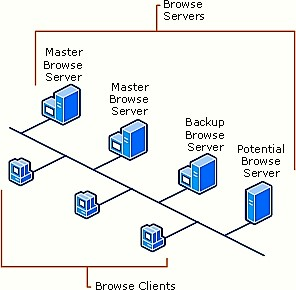
\includegraphics[width=5cm]{010_browser}
	\caption{Architettura Microsoft Windows Browser Protocol\label{fig:winBrowser}}
\end{figure}
Il nodo radice di tale struttura viene chiamato \textit{Domain master browser}(o anche \textit{Primary Domain Controllers: PDCs}), ed � responsabile della gestione delle liste di tutti i servers, una per ogni sotto-rete del dominio con all'interno un nodo \textit{Master browser}. Al di sotto del PDCs, uno per ogni sotto-rete, si trovano i \textit{Master browsers}, i quali si occupano di gestire le \qts{browse lists} del loro sotto-dominio di competenza ed inoltrarle al PDCs di sopra, e ai \textit{Backup Browsers} al di sotto. Proseguendo nella gerarchia, al di sotto troviamo appunto i \textit{Backup Browsers}, che diffondono individualmente ai computers che ne fanno richiesta le informazioni raccolte nelle liste dei Master Browsers. Se si rendesse necessario, ci sono dei nodi che vengono etichettati come \textit{Potential Browsers}, pronti a sostituire un eventuale Browser non pi� funzionante. In fine ci sono il resto dei nodi della rete chiamati \textit{Nonbrowsers}, che sono appunto il resto delle macchine che non sono in grado di diffondere o tenere traccia delle liste di Browsing, ma che fanno parte della rete e offrono/richiedono servizi. \\

Dopo aver verificato quali informazioni sono contenute nei pacchetti catturati, si sono denotati vari tipi di messaggi, tra cui: \textit{Browser Election request}, con i quali il protocollo si autogestisce, eleggendo il nodo pi� consono al compito da svolgere; \textit{Get Backup List Request}; \textit{'Local-Master'/Host/Request/'Domain-Workgroup' Announcement}, con i quali si rendono pubbliche indicazioni su come raggiungere le varie macchine e quali servizi offrono. Ci sono vari altri tipi di messaggi per questo protocollo, ma non ne sono stati catturati. Le informazioni che se ne possono ricavare dagli \textit{Announcement} sono decisamente rilevanti, identificando il nodo che le annuncia con un nome, che tipologia di macchina sia(workstation, server, ...), il produttore, ... e altri dettagli. 


\subsection{Multicast DNS-(Service Discovery)}
mDNS\cite{mDNS} � un protocollo che si pone a sostituzione di un normale DNS centrale, dove magari in una piccola rete non vi � la possibilit�/necessit� di averne uno. In pratica si occupa di risolvere i nomi locali, con estensione \qts{.local}, tramite una richiesta da parte dell'host ad un indirizzo multicast(IPv4 224.0.0.251 / IPv6 ff02::fb), porta UDP 5353, inviando un messaggio dello stesso formato delle query DNS, ed ottenendo risposta, sempre in multicast, da un qualsiasi dispositivo(solitamente chi possiede il nome richiesto) che conosce l'indirizzo IP corrispondente. \\
Avendo la stessa struttura del protocollo DNS, oltre che alla risoluzione dei nomi, mDNS implementa anche il meccanismo DNS-Service Discovery\cite{privMDNS}, il quale permette la scoperta di istanze con nome di servizi nella rete locale, usando le querys standard DNS. Ogni servizio � identificato tramite un \textit{nome composto}, in notazione.\qts{puntata} conforme al meccanismo gerarchico di nomi DNS, il quale � cos� suddiviso: \textit{Istanza.Servizio.Dominio}. \textit{Istanza} identifica univocamente il particolare dispositivo che offre il relativo \textit{Servizio}, che a sua volta identifica il Tipo specifico di servizio offerto e il protocollo usato, ed in fine il \textit{Dominio} riporta lo specifico dominio all'interno del quale il servizio � offerto (nel caso di mDNS � sempre \qts{\textit{.local}}).\\

Per quanto riguarda i vari Tipi di servizi offerti in rete, IANA fornisce una lista\cite{IANA} dei servizi ad oggi registrati, ed offre la possibilit� di registrarne di propri, ma � comunque possibile utilizzare anche tipi non registrati e proprietari, senza la necessit� di registrarne il nome.\\
\begin{figure}[h]
	\centering
	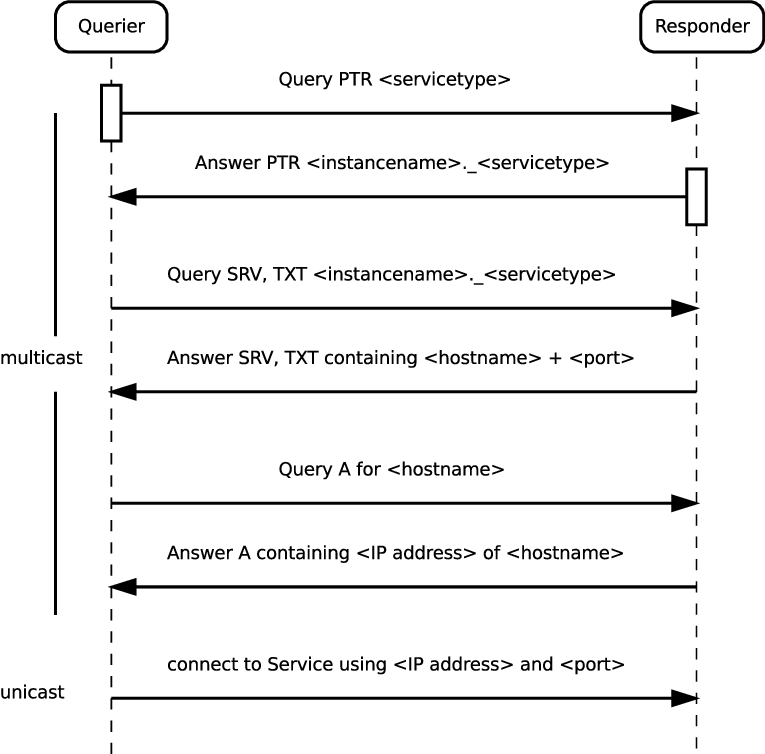
\includegraphics[width=5cm]{011_mdns_iter}
	\caption{Iter per il Service Discovery\label{fig:mDNS_iter}}
\end{figure}

Ogni dispositivo che vuole condividere/offrire un servizio, annuncia in multicast mDNS i record DNS-SRV e DNS-TXT. I record SRV riportano il nome, come descritto in precedenza, \textit{Istanza.Servizio.Dominio},e l'host con porta di destinazione a cui fare riferimento per richiedere il servizio. I record TXT sono opzionali, quindi non tutti i servizi annunciati li diffondono e non tutti i servizi dello stesso tipo rendono noti gli stessi campi, riportano alcuni dettagli del servizio offerto, e molto spesso, anche informazioni riguardo il dispositivo che si rende disponibile ad offrire il servizio. \\
Il dispositivo che invece vuole fare richiesta, usufruire, o semplicemente scoprire se il un dato servizio � reperibile, acquisisce la lista dei servizi disponibili effettuando delle query in multicast per ottenere record DNS-PTR, e richiedendo il nome del servizio del tipo: \textit{Servizio.Dominio}. Come risposta, se nella rete � presente un host che ha le informazioni richieste, viene inoltrato in multicast un messaggio mDNS contenente, oltre al PTR che indica il nome completo dell'istanza del servizio, vengono forniti anche i record REV ed eventuali TXT collegati citati in precedenza.\\

Fra tutti i vari protocolli di Multicast/Broadcast rilevati, mDNS ha catturato maggiormente l'attenzione, sia per quanto riguarda la quantit� di traffico generata, ovvero le molteplici query di discovery per i servizi presenti; sia per le informazioni specifiche contenute all'interno, che talvolta ha reso possibile di identificare, con una buona dose di affidabilit�, il tipo e modello dispositivo fisico con tanto di dettagli tecnici riguardanti i pezzi hardware che lo compongono, il software che in quel momento � in esecuzione, e molto altro.


\subsection{Dropbox LAN sync Discovery Protocol}
Dropbox, una delle applicazioni pi� usate per il servizio di cloud storage e file sharing tramite Internet, utilizza per la sua versione desktop un protocollo chiamato Dropbox LAN sync Discovery Protocol(oppure in breve \textbf{\textit{db-lsp-disc}}), con il quale incrementa la velocit� di sincronizzazione\cite{broadID} tra gli host che condividono le stesse cartelle all'interno della medesima rete locale. Questo inoltre evita anche che per ogni cartella condivisa, avvenga la sincronizzazione fra l'host che la condivide e i server di Dropbox, generando del traffico superfluo all'esterno della rete locale, e quindi limitando lo scambio di dati all'interno della LAN.\\

Questo meccanismo � reso possibile tramite lo scambio dei pacchetti db-lsp-disc fra gli host Dropbox, all'interno dei quali vi sono varie informazioni, tra cui: un identificatore unico, generato al momento dell'installazione, che identifica l'host; alcuni campi di utilit� come versione app, display name, e porta usata per lo scambio di dati; ed infine il campo pi� interessante, \textbf{\textit{namespaces}}, il quale riporta l'elenco di cartelle condivise in Dropbox con altri utenti. In realt�, Namespaces non riporta effettivamente l'elenco dei nomi delle cartelle, ma un'elenco di id unici che identificano le varie cartelle condivise. Questa � un'informazione molto preziosa, dato che pur non conoscendo nulla di un nodo della rete, se ne pu� rivelare le interazioni con altri dispositivi ad essa collegati, e quindi carpire le interazioni fra gli utilizzatori della rete locale.

\section{Panoramica del Lavoro}
Relativamente a questo lavoro di tesi, gli ultimi 2 protocolli si sono rivelati molto interessanti, fornendo informazioni decisamente \qts{riservate} e private, ma soprattutto troppo facilmente accessibili, essendo recapitate direttamente a qualsiasi dispositivo collegato alla LAN, interessato o meno, il quale si ritrova in modo completamente passivo tali dettagli.\\

Partendo da questa considerazione, � stato deciso di sviluppare un piccolo componente software che analizzi in automatico tutte queste informazioni e le raccolga in una struttura dati. Questa struttura dati racchiuder� ogni dettaglio dei relativi nodi utilizzatori di tali protocolli, rivelandone la natura, le \qts{abitudini}, gli applicativi software in esecuzione, e in alcuni casi anche il possessore del dispositivo e le interazioni con altri utenti/dispositivi connessi alla medesima rete locale. \\
Per la raccolta del traffico dati � stato utilizzato, come per lo studio del traffico della rete locale, l'applicazione Wireshark(e la relativa versione in-line T-Shark), rivelatosi lo strumento perfetto a tale scopo, dato che permette di catturare tutto il traffico che transita dalla scheda di rete del dispositivo sul quale � in esecuzione. Il traffico poi � stato filtrato eliminando tutti i pacchetti unicast, ottenendo quindi una cattura di soli  pacchetti Broadcast/Multicast.\\
Per la realizzazione del componente software, scritto in Python, � stato utilizzato un wrapper\cite{web:pyshark} di T-Shark, anch'esso scritto in Python, il quale permette di leggere i file di cattura precedentemente ottenuti, e accedere ai singoli pacchetti del file e quindi reperire le informazioni contenute all'interno dei singoli campi. 

\subsection{Funzionamento}
Di seguito verr� descritto il funzionamento dell'algoritmo che compone il software sviluppato per questo lavoro, tralasciando i dettagli tecnici nel prossimo capitolo, e limitandone la descrizione ad una panoramica completa.\\

La struttura principale � composta da un insieme di dispositivi, identificati univocamente dal loro MAC-Address, ognuno dei quali contiene: gli ultimi indirizzi IPv4 e IPv6 conosciuti(i quali ovviamente potrebbero essere cambiati da un'assegnamento dinamico), l'ipotetico possessore del dispositivo, la tipologia di dispositivo supposta a seguito dell'analisi, un elenco di \textit{alias} con i quali viene identificato il dispositivo, un elenco di tutti i servizi offerti dal dispositivo, rilevati tramite le informazioni contenute all'interno dei pacchetti mDNS, ed infine un campo che riporta tutte le informazioni raccolte dal protocollo Dropbox db-lsp-disc.\\

A sua volta, ogni Servizio � rappresentato da una struttura dati composta, contenente tutte le informazioni reperite a riguardo: nome completo (\textit{Istanza.Servizio.Dominio}) e le relative componenti del nome separate(utilizzate in fase di analisi dei vari dispositivi), il nodo \qts{target} al quale riferirsi per ottenere il servizio(e la relativa porta), e un'elenco di campi \textit{TXT} i quali riportano ulteriori dettagli relativi al servizio offerto, nonch� del dispositivo che lo rende disponibile.
\begin{figure}[h]
	\centering
	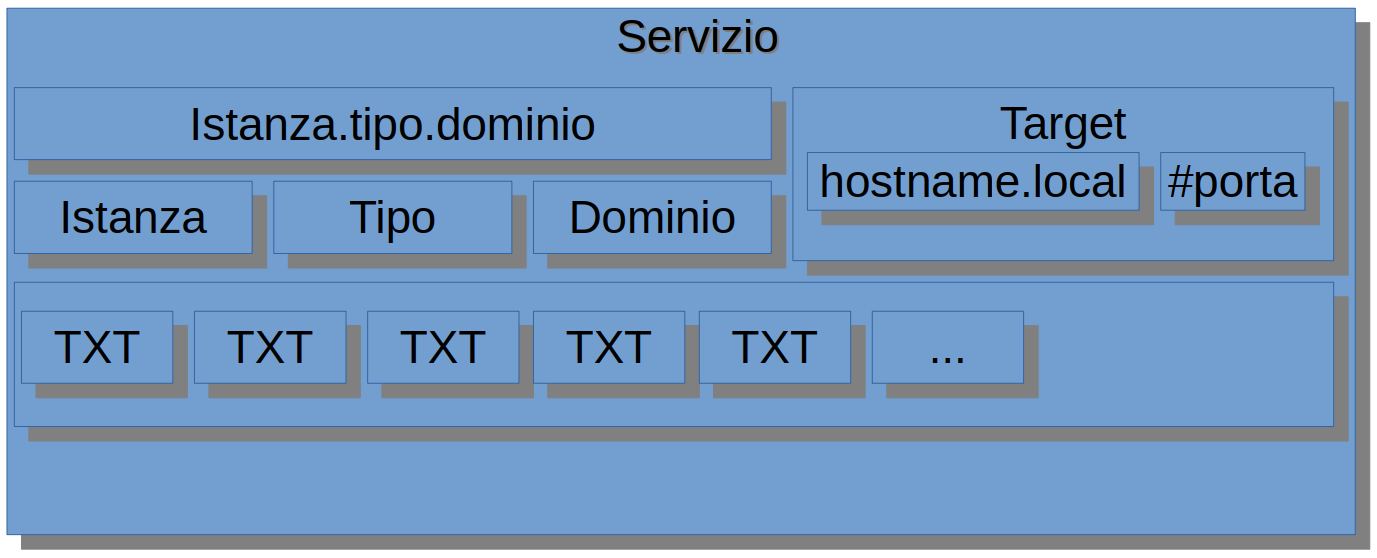
\includegraphics[width=\linewidth]{012_serviceMDNS}
	\caption{Struttura che racchiude informazioni riguardo un generico servizio\label{fig:serviceMDNS}}
\end{figure}

Per quanto riguarda il campo contenente informazioni Dropbox del dispositivo, viene rappresentata sempre come una struttura dati composta, che racchiude gli stessi campi dei pacchetti db-lsp-disc, e in particolare la lista dei Namespaces che quel nodo della rete ha annunciato nel corso della cattura.\\

In primo luogo, viene effettuata un'analisi e raccolta di dati rilevanti all'interno dei pacchetti mDNS, a seconda della quale viene aggiunto o meno un nuovo dispositivo nella struttura principale, e in seguito vengono raccolte le informazioni reperite dai pacchetti Dropbox, arricchendo le informazioni sui dispositivi gi� rilevati con lo studio mDNS precedente, oppure aggiunti nuovi dispositivi alla struttura.\\

L'analisi di un pacchetto mDNS\label{extract_mDNS_info} avviene a partire dal campo MAC-Address sorgente, che identifica il nodo che ha inviato il pacchetto, se presente il Layer mDNS, e in particolare la presenza di record di risposta\footnote{per questa analisi, � stato deciso di prendere come certa la presenza di un servizio solo se un dispositivo annuncia la presenza di tale servizio in un record \qts{answer}} alle query: qualora uno di questi campi venisse meno, l'analisi del pacchetto mDNS si interrompe.
Utilizzando quindi il MAC-Address del dispositivo, se ne verifica la presenza nella struttura principale: se gi� presente, viene riferita l'istanza precedentemente rilevata, altrimenti ne viene creata una nuova(ma NON ancora aggiunta alla struttura principale).\\
Dopo aver aggiornato l'eventuale indirizzo IPv4 o IPv6 del dispositivo(che magari potrebbe esser stato riassegnato), parte il vero e proprio studio del pacchetto mDNS. Per ogni record \qts{risposta}, viene verificato se appartiene ad uno dei tipi di record utili al nostro lavoro:
\begin{itemize}
	\item[\textbf{16}] Record TXT: viene creata una nuova istanza del servizio, identificata dal suo nome completo (Istanza.Tipo.Dominio) e ne vengono estrapolati tutti i campi TXT contenuti nel record.
	\item[\textbf{1}] Record A: analogamente ai record DNS, riporta la risoluzione di un nome in un indirizzo IPv4; tipicamente, il nodo della rete che lo annuncia � esso stesso il possessore di quell'indirizzo, assegnandogli quindi il nome riportato nel record; ma pu� anche accadere che non lo sia: in questo caso, si scansiona l'intera struttura dati principale alla ricerca di un device che ne riporti l'indirizzo IPv4, e in caso positivo, si assegna il nome a QUEL dispositivo, non a chi lo ha annunciato. 
	\item[\textbf{28}] Record AAAA: segue lo stesso ragionamento per i Record di tipo A, ma riportando la risoluzione di un nome in un indirizzo IPv6
	\item[\textbf{33}] Record SRV: vengono raccolte le informazioni contenute, quindi nome completo, nome suddiviso nei vari campi istanza tipo dominio del servizio, e l'host target al quale riferirsi. 
\end{itemize}
Possono essere presenti altri tipi di record, ma ai fini di questo lavoro di tesi, non contengono informazioni rilevanti, quindi vengono ignorati.\\

Pu� accedere per�, che il dispositivo che annuncia il servizio non sia effettivamente il provider di tale, ma semplicemente condivida questa informazione acquisita in precedenza. 
\begin{figure}[h]
	\centering
	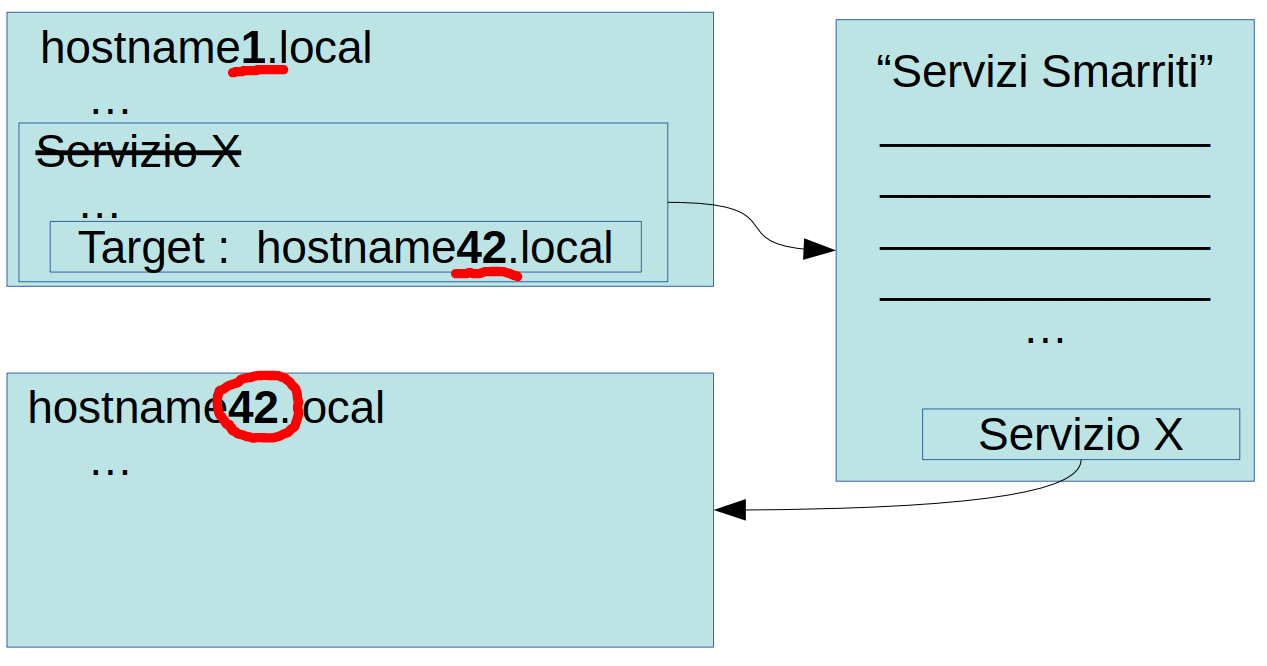
\includegraphics[width=\linewidth]{013_lostsrv}
	\caption{\qts{Servizio X} offerto dall'host 42, NON dall'host 1\label{fig:lostsrv}}
\end{figure}
Quindi, prima di aggiungere il nuovo dispositivo con tutti i servizi rilevati, si controlla che ogni servizio attribuito al nodo abbia come target il dispositivo che lo ha annunciato: se cos� non fosse, viene effettuata una ricerca nella struttura principale, verificando se esiste un nodo che effettivamente � il fornitore di tale servizio(host \textit{target}, o istanza del servizio); se non esistesse alcun dispositivo corrispondente, il servizio viene aggiunto ad una lista dove vengono raccolti tutte le istanze dei servizi i quali non hanno ancora trovato l'effettivo target al quale riferirsi. 
Questa lista verr� controllata ogni volta che viene identificato un nuovo host, assegnando quindi i servizi al proprio fornitore. L'esempio in Fig. \ref{fig:lostsrv} riporta un generico \qts{\textit{Servizio X}} che viene annunciato dal dispositivo con \textit{hostname1.local}, ma che in realt� viene offerto dal nodo che ha \textit{hostname42.local}.\\
In conclusione del recupero dati dal pacchetto mDNS, viene verificato che il dispositivo contenga informazioni rilevanti nella sua struttura: ovvero gli sia stato attribuito almeno un nome/alias che lo identifichi, o per lo meno sia l'effettivo fornitore di almeno un servizio. In caso positivo, il nodo viene aggiunto alla struttura principale.\\

Per quanto riguarda la raccolta di informazioni di un pacchetto Dropbox, il procedimento � semplificato, e si limita a raccogliere dati dai campi del relativo pacchetto, ed assegnare tali informazioni al dispositivo nella rete locale che lo ha inoltrato.\\
Come per mDNS, per ogni pacchetto db-lsp-disc, se ne recupera l'indirizzo MAC e quello IP, se ne verifica la presenza nella struttura principale, e nel caso in cui non sia gi� stato rilevato, viene creata una nuova istanza di dispositivo. Proseguendo, si recuperano tutti i campi del Layer db-lsp-disc: \text{host-int}, version, displayname, port, namespaces, creando un nuovo campo del dispositivo per raccoglierle se non presente, o aggiornando la lista dei namespaces altrimenti.\\

Conclusa la fase di Raccolta Dati, inizia la fase di elaborazione delle informazioni raccolte, parte centrale di questo lavoro. Come per la precedente fase, vengono effettuate 2 analisi separate: una per le informazioni raccolte dal protocollo mDNS, e l'altra per lo studio delle informazioni Dropbox.\\
Grazie allo studio dei record mDNS, per quasi tutti i nodi della rete che hanno annunciato dei servizi, si riesce a ricavare con buona precisione la natura del dispositivo che ne ha dato disponibilit�. 
Per etichettare gli host, � stato deciso di suddividerli in Macro-Categorie, le quali coprono in pratica la totalit� dei tipi di dispositivi attualmente in circolazione: 
\begin{itemize}
	\item[Workstation] Il gruppo pi� generico dei dispositivi. Qui vengono raccolti tutti i nodi che spaziano fra Personal Computer Desktop, Laptop, Server, \dots e affini.
	\item[NAS] \'E una specializzazione del gruppo Workstation, e indica tutte le macchine adibite alla funzione di Network Attached Storage; sono quindi tutti quei dispositivi che archiviano e condividono dati, da file, immagini, musica, e altro.
	\item[Mobile] In questa sezione vengono raccolti tutti i dispositivi mobili, quindi principalmente Smatphones, Tablets, che essi siano Apple o Android.
	\item[Printer] Questo gruppo racchiude tutti quei nodi della rete che si possono categorizzare come Stampanti, Scanner, o Stampanti-Multifunzione, quindi tutti quei dispositivi usati per le utilit� d'ufficio.
	\item[Media] Questo gruppo indica tutti quei dispositivi utilizzati per la riproduzione di Media quali: la musica, video, foto, e qualsiasi cosa inerente all'intrattenimento in formato digitale.
\end{itemize}

Per suddividere i nodi nelle suddette categorie, sono stati utilizzati alcuni Tipi Specifici di servizi annunciati nei record mDNS, supponendo con una buona dose di certezza che dati tipi potessero essere annunciati, con buona probabilit�, solo da determinati tipi di dispositivi.\\

Lo studio per attribuire un'identit� ad un dispositivo parte con la l'analisi delle tipologie di servizi annunciati dallo stesso. In primo luogo si va alla ricerca di un particolare servizio fittizio annunciato dai dispositivi Apple chiamato '\_device-info', il quale non annuncia un servizio vero e proprio, ma riporta i campi TXT \textit{model} e opzionalmente \textit{osxversion}: se presenti, e a meno di falsificazione e diffusione di informazioni errate da parte dell'host, si identifica con certezza e precisione la natura del dispositivo grazie a questi campi, e con l'aiuto di un dizionario riportante quasi la totalit� dei numeri di modello dei rispettivi prodotti e versioni del sistema operativo Apple, si viene a conoscenza delle specifiche complete Hardware e Software della macchina. Questa, a mio avviso, si rivela l'informazione pi� delicata fa tutte quelle raccolte, in quanto fornisce delle specifiche veramente dettagliate e private del nodo, fornendo ad intrusi/ospiti nella rete eventuali punti deboli per compromettere il corretto funzionamento o pi� semplicemente informazioni sulle scelte Hardware e Software dell'azienda in cui si trova.\\

Lo studio procede scorrendo l'elenco di tutti gli alias e nomi mnemonici che sono stati attribuiti al nodi stesso(nome.local) o all'istanza del determinato servizio che offre(la sezione \textit{Istanza} del nome del servizio). Per prima cosa si va alla ricerca degli alias del tipo \textit{nome.local}, che solitamente riporta una stringa composta, creata dalla combinazione del nome che l'utente d� alla macchina, e l'aggiunta di stringhe mnemoniche assegnate dal Sistema Operativo usato dall'utente. 
Questo spesso porta a creare nomi che riconducono facilmente alla natura del dispositivo, riportando keyword del tipo: 'MacBook-Pro' o 'Computer', oppure 'iPhone' e 'Android', o ancora 'Time Capsule'.\\
\begin{figure}[t]
	\centering
	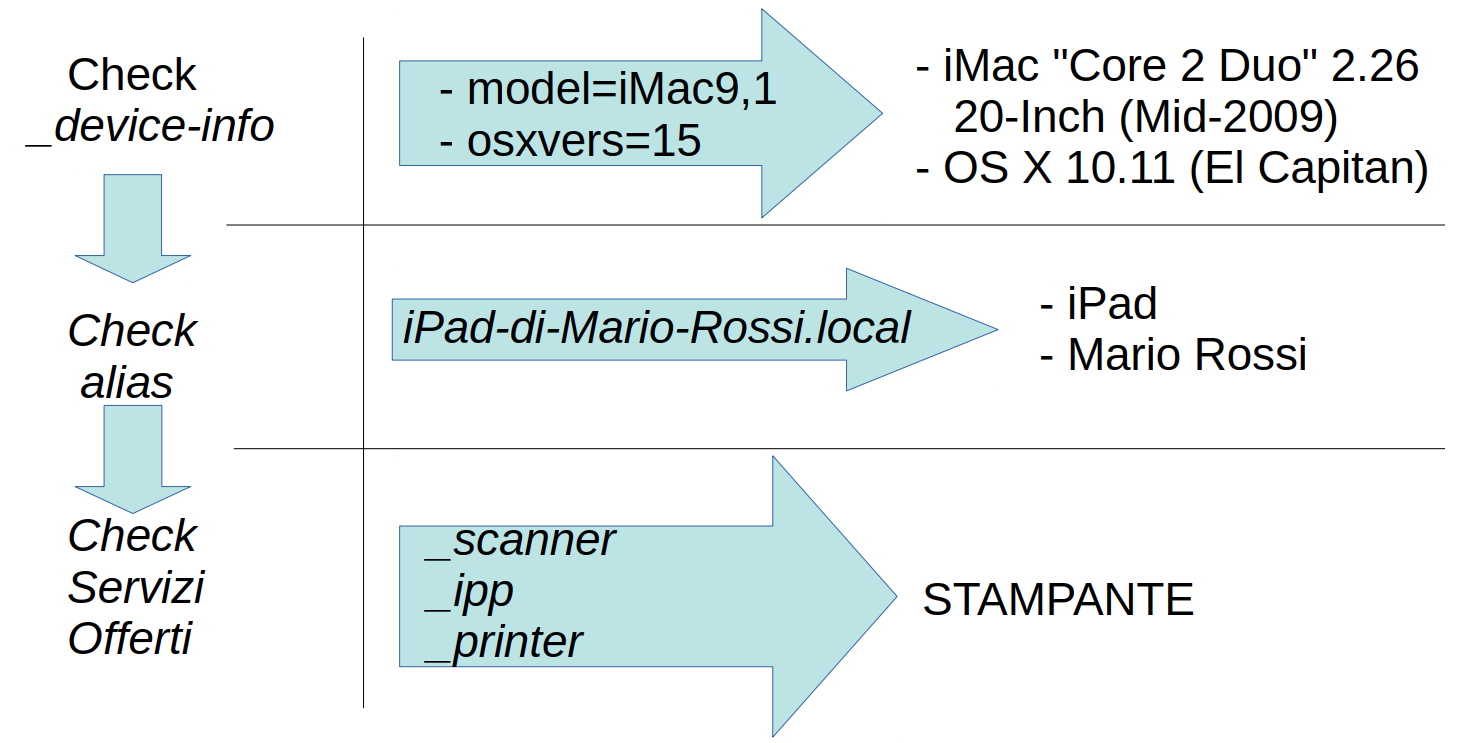
\includegraphics[width=\linewidth]{014_mdns_study}
	\caption{Iter dell'analisi di un dispositivo\label{fig:mdns_study}}
\end{figure}

Queste informazioni, se pur con un'alta dose di incertezza, sono un buon punto di partenza per supporre il tipo di dispositivo che � stato rilevato. Ovviamente, fra tutte le informazioni raccolte e come appena accennato, questi sono dati da considerarsi non del tutto affidabili, dato che per un utente medio e consapevole, sarebbe fin troppo semplice modificare o attribuire un nome che depisti la corretta identificazione del dispositivo. Tuttavia, nell'analisi di questi nomi, si � notato che l'utente medio tende ad ignorare questo dettaglio, anzi, spesso come nome che identifichi il dispositivo utilizza il suo vero nome, talvolta seguito anche da cognome, fornendo anche questa personalissima informazione riguardo al possessore del dispositivo.\\
Recuperare questo dato � reso possibile grazie a tutti gli utenti che come nome del dispositivo utilizzano una stringa del tipo 'Marios-iPhone.local'(in Inglese), oppure 'MacBook-Pro-di-Maria-Rossi.local'(in Italiano), dando quindi la possibilit� di ipotizzare il Nome e Cognome del possessore del dispositivo.\\

In fine, avviene l'analisi vera e propria sui servizi annunciati dal nodo, suddivisi per categoria, e ad ognuno dei quali � attribuito un \textit{grado di affidabilit�} che spazia dal 1(completamente inaffidabile) al 9(completamente affidabile), con il quale si cerca di collocare il dispositivo in una delle Macro-Categorie sopra citate. Per ognuno dei servizi annunciati, si verifica quale categoria di dispositivi lo pu� aver diffuso, e con quale grado di affidabilit�. Al termine di tale processo, si verifica qual'� la Categoria la quale ha la maggiore affidabilit�, e se non � stato rilevato il record \_device-info sopra descritto, il dispositivo, dopo un'ultimo controllo, viene categorizzato.\\
\begin{table}[h]
	\centering
	\begin{tabular}{lcl}
		\multicolumn{1}{c|}{Servizio}            & Rate                   & \multicolumn{1}{|c}{Descrizione}                    \\ \hline
		\multicolumn{1}{l|}{\_spotify-connect} & \multicolumn{1}{c|}{7} & \multicolumn{1}{l|}{Device running Spotify}        \\ \hline
		\multicolumn{1}{l|}{\_airplay}         & \multicolumn{1}{c|}{6} & \multicolumn{1}{l|}{Device running Airplay}        \\ \hline
		\multicolumn{1}{l|}{\_amzn-wplay}      & \multicolumn{1}{c|}{9} & \multicolumn{1}{l|}{Amazon Firestick}              \\ \hline
		\multicolumn{1}{l|}{\_appletv-v2}      & \multicolumn{1}{c|}{9} & \multicolumn{1}{l|}{Apple TV}                      \\ \hline
		\multicolumn{1}{l|}{\_atc}             & \multicolumn{1}{c|}{6} & \multicolumn{1}{l|}{Device sharing iTunes Library} \\ \hline
		\multicolumn{1}{l|}{\_daap}            & \multicolumn{1}{c|}{8} & \multicolumn{1}{l|}{Digital Audio Access Protocol} \\ \hline
		\multicolumn{1}{l|}{\_googlecast}      & \multicolumn{1}{c|}{9} & \multicolumn{1}{l|}{GoogleCast}                    \\ \hline
		\multicolumn{1}{l|}{\_nvstream}        & \multicolumn{1}{c|}{9} & \multicolumn{1}{l|}{NVIDIA Shield}                 \\ \hline
	\end{tabular}
	\caption{Esempio di classificazione pe la categoria MEDIA\label{tab:class1}}
\end{table}

Prima di attribuire il nodo ad una specifica categoria, viene effettuato un'ultimo controllo, dovuto ad un comportamento anomalo riguardo l'annuncio di alcuni servizi, rilevato in fase di Test. Alcuni nodi della rete annunciavano servizi riportando nella sezione del nome \textit{Istanza} il carattere \qts{\text{@}}, nello specifico, la stringa era della forma: \qts{\textit{nome-disp-1 @ nome-disp-2}}. Dopo una rapida verifica, si � raggiunta la conclusione che ad offrire il servizio annunciato non era chi lo annunciava, ma bens� un'altro dispositivo collegato(per la totalit� stampanti) alla macchina che lo annuncia e che magari non possiede l'accesso alla rete per mancanza di permessi o, pi� probabile, essendo sprovvisto di scheda di rete. \\
Per identificare queste situazioni, prima di dare la conferma, si ricerca nel nome il carattere @, e si identifica il dispositivo, per esempio, non come una stampate, ma bens� come un \text{dispositivo che condivide una stampante}, aumentando quindi il grado di precisione del programma e riportando la corretta informazione.\\

Conclusa l'elaborazione delle informazioni ottenute dai pacchetti mDNS, si prosegue con l'analisi delle interazioni fra i dispositivi connessi alla rete locale. Riprendendo i dati contenuti nei pacchetti Dropbox, per ogni dispositivo che abbia trasmesso messaggi db-lsp-disc, si controlla se condivide nel proprio elenco di namespaces delle cartelle con altri nodi della rete locale. In caso positivo, si crea una lista associata al dispositivo che riporta tutti i nodi con cui condivide una o pi� cartelle Dropbox, creando cos� un grafo che rappresenta le interazioni fra i dispositivi e quindi fra gli utenti che usufruiscono della rete locale.\\
Questo a sua volta rivela anche la rete sociale degli utenti, supponendo che se persone condividono delle cartelle, � molto probabile, se non certo, che si conoscano, o per lo meno abbiano una qualche sorta di interessi o fini in comune, che siano per lavoro o per hobby.\\

\section{Pro e Contro Soluzione}
Analizzando nel complesso questo lavoro di tesi, si possono notare dei vantaggi e degli svantaggi nelle scelte progettuali ed implementative che adesso andremo ad analizzare.\\

Il primo argomento di discussione da affrontare � il punto in cui ci poniamo per raccogliere i dati da analizzare per lo studio della rete: la scheda di rete di un singolo nodo collegato alla stessa. Ovviamente questo ci pone in grande svantaggio e delle grosse limitazioni, e in particolare, ci nega l'accesso a tutti quei pacchetti unicast che non verranno mai inoltrati al nodo designato all'ascolto dei pacchetti. Per permettere l'intercettazione completa del traffico, ci si dovrebbe porre, come punto di raccolta del traffico, in uno snodo centrale della rete, come per esempio un accesspoint, uno switch o un router interno. Indubbiamente ci darebbe la visione completa del traffico, ma questo comporterebbe non poche difficolt� logistiche nell'avere accesso a tali punti di snodo. D'altra parte quindi, questa scelta progettuale comporta una maggiore facilit� nel recupero dei pacchetti che transitano nella rete locale, richiedendo quindi il semplice accesso a quest'ultima. Infatti uno degli scopi principali di questo lavoro � dimostrare la semplicit� con cui reperire informazioni private dei dispositivi che vi risiedono, e come queste siano accessibili a chiunque, con il minimo sforzo: necessitando semplicemente di leggere le informazioni che ci vengono recapitate, non andandole a cercare o compromettendo la sicurezza e quindi superando i meccanismi di protezione di un dispositivo.\\

Un'altro punto sul quale discutere � l'utilizzo del nome mnemonico di una macchina, \textit{hostname}, che se ne fa in questo lavoro per supporre la natura del dispositivo, e pi� in generale, l'affidabilit� delle informazioni reperite all'interno dei pacchetti. Nel mondo dell'informatica qualsiasi cosa � modificabile e \qts{ricreabile}, tanto pi� i pacchetti e le informazioni reperibili all'interno della rete. Basti pensare alla possibilit� di formare pacchetti manualmente, seguendo gli standard dei protocolli che si vogliono imitare: si ottengono delle informazioni prodotte non dal software che implementa il protocollo, ma pacchetti che seguono il medesimo standard di layout per i campi, e che ne contengono informazioni non generate per la loro effettiva veridicit�.\\
Tanto pi� � probabile che un utente accorto e consapevole di quanto siano vulnerabili le informazioni che attraversano le reti, potrebbe decidere di associare un nome al proprio dispositivo che depisti un'analisi superficiale che tenti di scoprirne il tipo e le componenti. Basti pensare, per esempio, ad un utente che chiama il proprio \textit{Smartphone Apple iPhone} con il nome \qts{\textit{Android}}, o viceversa.\\
Tuttavia, al termine del nostro studio e validazione dei risultati, si � riscontrata l'abitudine opposta da parte dell'utente medio: ovvero quella di non modificare affatto i nomi dei dispositivi, anzi, cercando di attribuirgli nomi ancor pi� evocativi e dettagliati riguardo la tipologia di dispositivo, rendendoli quindi, s� pi� riconoscibili dall'utente umano, ma anche facilmente identificabili da un applicativo software che ne estrapola le keyword e lo identifica. Gli esempi pi� rilevanti sono, oltre a quasi la totalit� dei i dispositivi Apple che siano mobile o PC, sono stati nomi del tipo: nomedinodo\textit{NAS}, o ancora nomedinodo\textit{PC} e nomedinodo\textit{DESKTOP}, e cos� via.\\
Come validazione di questo fatto, oltre che la verifica effettiva sulla tipologia del dispositivo, ci vengono in aiuto tutti i servizi annunciati tramite mDNS, e che quindi ne aumentano la precisione nell'identificare correttamente la categoria da attribuire al dispositivo.\\

Strettamente collegato al punto precedente, un'altro argomento di questo lavoro sul quale discutere � l'affidabilit� e la precisione con la quale si attribuisce una categoria ad un dispositivo, e se ne identifica quindi la tipologia. Al netto dell'incertezza dovuta alla possibilit� di modificare i pacchetti distribuiti in rete, accennata in precedenza, si suppone che se un dispositivo annuncia un dato servizio, effettivamente � in grado di offrirlo.\\
Per quanto riguarda la categorizzazione, la scelta concettuale � stata la seguente: attribuire i servizi pi� evocativi e discriminanti possibile ad ogni categoria di dispositivi. Ad esempio, se un dispositivo annuncia direttamente il servizio di stampa, scanner, o altro inerente a tale branca di servizi, � ovvio che il dispositivo non pu� essere uno Smartphone, un Laptop/Notebook o ancora un server: non ne ha fisicamente gli strumenti per offrirli! O ancora, se un dispositivo offre un servizio utilizzato unicamente da un'applicazione per Mobile, ovviamente non potr� essere un Server o una stampante. Ulteriori discussioni sono rimandate nelle pagine successive, nella sezione in cui si discute la validazione del lavoro software prodotto.

	%%%%%%%%%%%%%%%%%%%%%%%%%%%%%%%%%%%%%%%%%%%%%%%%%%%%%%%%%%%
% Capitolo 3

\chapter{Stato dell'Arte}
\label{ref:Arte}

Con l'avvento di tecnologie come Zeroconf, alla ricerca quindi di rendere indipendenti ed automatizzate le interazioni e collaborazione fra i dispositivi e le applicazioni che vi sono in esecuzione, il traffico Broadcast e Multicast � diventato sempre pi� diffuso, e con lui anche gli studi che sono stati approntati per migliorarne l'efficienza, l'affidabilit�, la fruibilit�, nonch� analisi atte a comprenderne maggiormente la natura delle meccaniche che vi troviamo alla base.\\
Nell'elaborazione di questo lavoro di Tesi mi sono ritrovato a visionare numerosi studi a riguardo, che similmente, o con approccio completamente diverso, hanno analizzato sotto vari aspetti il traffico Broadcast e Multicast diffuso nelle reti locali.

\section[z2z]{Discovering Zeroconf Services\\ Beyond Local Link\cite{z2z}}
Questo altro lavoro parte da alcune considerazioni sulla tecnologia \textit{Zeroconf}, in particolare alla limitazione sull'utilizzo di quest'ultima all'interno della rete locale per mezzo di comunicazione multicast. \'E stato sviluppato un applicativo chiamato \textit{Zeroconf-to-Zeroconf Toolkit} (z2z), nel tentetivo di realizzare a un'architettura ibrida che combinasse la semplicit� di utilizzo di Zeroconf con la scalabilit� di una rete peer-to-peer basata su DHT. \\Z2z connette pi� sottoreti Zeroconf usando OpenDHT, estendendo la raggiungibilit� delle applicazioni abilitate all'utilizzo di Zeroconf al di l� dei link locali. Inoltre, fornisce un framework  sul quale basarsi per costruire una soluzione globale di service discovery basata su Zeroconf.\\
Considerando l'enorme e crescente utilizzo di Zeroconf, si pu� notare che sempre pi� applicativi ne fruiscono, aumentando di molto il numero, ma soprattutto la tipologia di servizi offerti tramite questa tecnologia. Questo ha portato ad una considerazione: se l'utilizzo fosse limitato al processo di discovery di stampanti e dispositivi locali, non ci sarebbe alcun problema, e rivelandosi un meccanismo pienamete utilizzato. Ma ad oggi ci sono servizi come applicazioni di chat(per esempio \textit{iChat} di Apple), i quali sono limitati da questa restrizione della rete locale: sarebbe molto pi� consono permettere alla comunicazione fra gli utilizzatori di Zeroconf di interagire anche con altre reti locali, mantenendo comunque tutti i vantaggi riguardo la semplicit� di utilizzo.\\
Questo lavoro di estensione di Zeroconf � ispirato dalle recenti innovazioni nel campo di ricerca riguardo le reti peer-to-peer, tra cui le reti strutturate-sovrapposte p2p basate sulle  \textit{Distributed Hash Tables}(DHT), divenute popolari come sotto-strati sistemi distribuiti a livello globale. Le reti DHT sono caratterizzate da un efficiente algoritmo che mappa stringhe arbitrarie in uno specifico nodo di una rete e di produrre path di routing efficienti composti da un numero limitato di passaggi fra un nodo ed un'altro. Il mapping � deterministico e uniformemente distribuito, e questo permette efficienti implementazioni di numerosi servizi di scala globale come il \textit{file-sharing} e \textit{multicast-overlay}.\\
Queste considerazioni sono state finalizzate in questo altro lavoro con il connettere sotto-reti Zeroconf utilizzando reti DHT, in particolare OpenDHT, un servizio DHT pubblicamente accessibile. Quindi, un processo \textit{z2z} in esecuzione in una sotto-rete esporta i servizi Zeroconf localmente disponibili in OpenDHT. Un'altra istanza di un processo \textit{z2z} in esecuzione in un'altra sotto-rete controlla i servizi esportati in OpenDHT e li importa nella propria rete locale, diffondendoli come se fossero originari di quella LAN. Tali servizi, agli occhi delle applicazioni, sono indistinguibili da quelli veramente annunciati localmente, e sono quindi assimilati dalle applicazioni che utilizzano Zeroconf come nulla fosse, non modificando quindi il proprio comportamento.\\	   

Questo lavoro mette ancor pi� in risalto quanto le informazioni diffuse tramite questi protocolli siano veramente delicate, in quanto estendendo l'area di diffusioni a pi� sotto-reti esterne si aumenta il numero di potenziali \qts{ascoltatori malintenzionati} che potrebbero usare i dati privati cos� ottenuti per i propri fini. 

\section[Privacy mDNS]{Privacy Implications of mDNS\cite{privMDNS}}
Similmente al nostro studio, questo altro lavoro tratta appunto le informazioni contenute nei messaggi mDNS e DNS-SD che circolano nelle reti locali, approfondendo in particolare le implicazioni che hanno rispetto alla privacy degli utilizzatori di applicazioni che ne fruiscono dei vantaggi.\\
La differenza dal nostro elaborato sta anche nella parte implementativa per quanto riguarda lo strumento per la raccolta e l'analisi delle informazioni ottenute dai record mDNS. Quest'altro strumento � stato realizzato con 3 tools aventi compiti distinti: il primo, chiamato \textit{Logger}, ha il compito di richiedere e scoprire la presenza di servizi annunciati tramite mDNS nella rete locale, stimolando la comunicazione dei dispositivi connessi effettuando delle querys attive per verificarne la presenza; un \textit{Database Server} il quale raccoglie le informazioni ottenute a seguito delle querys, archiviandole permanentemente in un Database; un \textit{Analyzer}, il quale recupera le informazioni raccolte nel Server Database e le analizza, filtrandole per tipo di servizio/protocollo, e producendo l'effettivo studio dei dati raccolti. \\Le comunicazioni fra il Server e gli altri 2 componenti sono state implementati tramite comunicazioni REST, quindi il server offre una semplice interfaccia supportata dal protocollo HTTP con la quale interagire. A tale scopo, � stato utilizzato il framework Spring-Boot\cite{SPRBOOT}, che � un'implementazione REST.\\

Per quanto riguarda l'analisi, questo altro lavoro si � concentrato non tanto sulla scoperta di informazioni del singolo dispositivo, ma bens� sull'analisi e lo studio dei singoli servizi/protocolli annunciati all'interno della rete, disinteressandosi dallo scoprire le caratteristiche del singolo nodo. Un'altra differenza nell'analisi sta nel fatto che � stato effettuato uno studio separato fra varie tipologie di rete(Privata, Semi-Pubblica, Pubblica/Open), confrontando poi le varie tipologie di protocolli rilevate, e in quali percentuali nelle une rispetto che nelle altre. Il nostro lavoro invece si � specializzato nel rivelare identit� del dispositivo e, in alcuni casi, del possessore, fruendo delle sole informazioni reperibili in modo completamente passivo, e quindi non generando alcun tipo di traffico per stimolare l'invio di messaggi mDNS.

\section[Broadcast Data Study]{How Broadcast Data Reveals Your Identity and Social Graph\cite{broadID}}
Un'altro studio simile a questo lavoro di tesi � l'analisi del traffico Broadcat e Multicast effettuato dall'Universit� di Scienze Applicate di Asburgo, la quale ha ampliato lo studio arricchendolo con l'aggiunta di altri protocolli oltre a mDNS e Dropbox, il tutto incrociando i risultati con i Databases interni dell'universit�, identificando con precisione gli utenti, rivelandone completamente l'identit�.\\
Inoltre, il team di Asburgo si � basato su di una quantit� di dati molto pi� elevata rispetto al nostro studio, se pur limitandosi alla rete interna all'universit�: ben 40GB di traffico broadcast per ogni 6 mesi, e per un totale di 2 semestri di monitoraggio.\\
Oltre ai protocolli usati in questo lavoro, sono stati analizzati e sfruttati per la raccolta di ulteriori informazioni, i pacchetti generati da protocolli come SSDP, LLMNR, e NetBIOS. Questo gli ha reso possibile accrescere il numero di informazioni ottenute, con dettagli che spaziano fra ulteriori nomi degli host grazie a NetBIOS, alla lingua parlata dall'utente(Inglese, Tedesco, ...) grazie sempre al parsing del nome dei nodi del tipo \qts{\textit{iPhone von John Doe}}, il quale indica chiaramente le origini Tedesche dell'utente grazie alla keyword \qts{von}.\\
In fine, questo altro studio ha incrociato gli hostnames raccolti con i dati nel server LDAP dell'universit�, il quale contiene l'intero elenco di tutti i nominativi(nome e cognome), matricole, email, corsi tenuti/seguiti, status(studente, insegnate, personale...) di tutti gli utenti registrati e facenti parte dell'universit�. Per disambiguare alcuni \qts{omonimi} fra i vari nomi estratti dagli hostnames rilevati e i nomi degli utenti registrati, sono stati utilizzati anche il timestamp del momento della cattura delle informazioni, incrociandoli con i corsi seguiti dagli utenti, tenuti dai professori, o ancora con i turni di lavoro del personale, associando al dispositivo, nella maggior parte dei casi, il corretto proprietario. 

\section{Arginare il problema della Privacy}
Presa coscienza dei problemi che comporta la trasmissione in chiaro delle informazioni diffuse tramite Broadcast/Multicast, e quindi mDNS in particolare, sono stati approntati numerosi studi atti ad aggiungere un layer di sicurezza e information-hiding, rendendo tali dati fruibili soltanto agli utenti autorizzati.\\
Fra i vari lavori a riguardo, mi sono trovato ad osservarne alcuni, che di seguito saranno brevemente accennati.\\

Daniel Kaiser e Marcel Waldvogel, autori dell'elaborato \textit{Adding Privacy to Multicast DNS Service Discovery}\cite{privAdd1}, hanno ideato un'estensione nelle comunicazioni DNS-SD per la privacy, la quale permette di nascondere tutte le informazioni sensibili dei record che annunciano i servizi offerti da un host, non necessitando alcuna modifica nella configurazione della rete, limitandosi all'aggiunta di una piccola fase di \textit{pairing} iniziale.\\
Dopo la solita analisi di quali informazioni si possono ricavare dai messaggi DNS-SD, � stato deciso di sviluppare uno strumento che, tramite tecniche di crittografia, non appesantisse il protocollo con l'aggiunta di overhead computazionale, e inoltre non comprometta il regolare funzionamento delle applicazioni che usufruiscono del protocollo di Service Discovery, ma che riuscisse comunque a fornire l'oscuramento delle informazioni per tutti gli host non autorizzati. Per permettere ci�, � comunque necessaria una piccola fase iniziale di \textit{pairing} fra i dispositivi che vogliono condividere/richiedere il permesso per l'utilizzo del Servizio: questo � stato implementato tramite lo scambio di informazioni per mezzo di un canale sicuro/esterno alla rete locale, come ad esempio Bluetooth, un QR-Code o NFC, o ancora una email crittografata o un SMS. In questa fase, i 2 host si scambiano tutte quelle informazioni necessarie a decrittare i dati diffusi in rete, rendendo personalizzabile, da parte dell'host che offre il servizio, la decisione di condividere o meno informazioni con gli altri nodi della rete.\\

In un'altro lavoro, \textit{User-Friendly, Versatile, and Efficient Multi-Link DNS Service Discovery}\cite{privAdd2} � stato elaborato un modo per fornire capacit� multi-link e scalabilit� per DNS-SD pur mantenendo la sua semplicit� d'uso e l'afficienza. Viene quindi proposta una soluzione Stateless-DNS (DNS-SD/sDNS), che permetta l'autoconfigurazione di Service Discovery spazi di nomi arbitrari, largamente indipendenti dal layout fisico della rete, sfruttando la loro tecnica \textit{statles DNS} e l'algoritmo di consensus Raft\\
Non mi sono addentrato nei dettagli di quest'ultimo studio, quindi per ulteriori informazioni riferirsi alla bibliografia di questo elaborato.

	%%%%%%%%%%%%%%%%%%%%%%%%%%%%%%%%%%%%%%%%%%%%%%%%%%%%%%%%%%%
% Capitolo 4

\chapter[Implementazione]{Dettagli di Implementazione}
\label{ref:Implementazione}

Questo lavoro di tesi, nello specifico lo sviluppo del componente software, � stato reso possibile, oltre a Wireshark, grazie ad un wrapper di tshark scritto in python chiamato \textit{pyshark}, il quale fornisce delle funzioni d'interfaccia che permettono di catturare/leggere file di cattura, ed accedere ai campi che compongono i vari pacchetti, estraendo informazioni utili.\\
Lo strumento software invece � stato sviluppato in Python nella versione 3, ed � composto da 4 moduli: DropBox\_utils.py, classFrames.py, discriminators\_sets.py, run\_test.py, i quali verranno descritti in dettaglio in questo capitolo.\\

\subsection{\textit{WireShark} (\textit{TShark})}
Software\cite{web:wireshark} Open-Source che permette di catturare il traffico di dati che transita sulla scheda di rete della macchina sulla quale viene mandato in esecuzione, senza la necessit� porsi in punti di snodo \qts{centrali}, come Router o Accesspoint. Questo limita molto il traffico dati catturabile, ma permette comunque di ottenere informazioni su tutti i pacchetti inviati/ricevuti a altri dispositivi in Unicast della macchina sulla quale � in esecuzione Wireshark, ed quindi anche tutti i messaggi inviati/ricevuti in Broadcast/Multicast, che per i nostri scopi � pi� che sufficiente.
Wireshark riesce a \qts{comprendere} la struttura di diversi protocolli di rete, � in grado di individuare eventuali incapsulamenti, riconosce i singoli campi e permette di interpretarne il significato. 
Per la cattura dei pacchetti Wireshark non dispone di proprio codice, ma utilizza libpcap/WinPcap, quindi pu� funzionare solo su reti supportate da libpcap o WinPcap. \\
Un'altra caratteristica utile ai nostri obiettivi � quella di non rendere visibile al resto della rete che si sta analizzando del traffico dati: questo offre ottimi spunti di riflessione riguardo la privacy di questi dati, in quanto non � possibile identificare chi li stia ricevendo(in pratica tutti i nodi della rete), come vengano usati, e quando questi dati vengono elaborati.\\
 
\textit{Tshark}, nello specifico, � una utility \qts{a linea di comando} di Wireshark, che utilizza quindi il core del programma principale, offrendo le medesime funzionalit�, ed � principalmente usato in tutti quei casi in cui non si necessita di interfaccia grafica, e si richiede output standard(in-line)

\subsection{\textit{Pyshark}\cite{web:pyshark}} 
Wrapper per tshark, reperibile sulla piattaforma GitHub.\\
Non � propriamente un dissector, come molti altri, ma si limita a usare la funzionalit� di tshark di esportare XMLs per usare il loro parsing. Questo package permette di estrarre informazioni sia da file di cattura, sia da \qts{catture Live}, utilizzando tutti i dissector di wireshark installati sulla stessa macchina.\\
Ai fini di questo lavoro, � stato usato il parsing su file di cattura precedentemente ottenuti, in quanto un analisi della rete il pi� completa possibile si ha soltanto dopo un certo quantitativo di pacchetti catturati.\\
Ogni pacchetto viene rappresentato da una struttura dati chiamata \textit{Packet}, la quale suddivide il pacchetto in \textit{Layer}, accessibili tramite indice o \qts{nome}. Un \textit{Layer} contiene tutti i campi che un \qts{layer di un pacchetto} possiede, sotto forma di \textit{LayerField}. In fine, un \textit{LayerField} contiene, nel caso in cui il campo contenga una singola informazione, tutti i dati contenuti in un campo di un layer di un pacchetto; nel caso in cui il campo contenga un gruppo di informazioni, per lo pi� strutturate a sua volta, tale campo viene suddiviso in pi� \textit{LayerField}s, ognuno dei quali contiene una lista che raccoglie tutti i sotto-campi di un determinato tipo. Per chiarire, un esempio verr� presentato in seguito, durante la descrizione dell'implementazione del processo che estrae informazioni mDNS da un pacchetto.

\subsection{Python 3}
Per lo sviluppo del tool di analisi, � stato scelto come linguaggio Python nella versione 3,un linguaggio multi-paradigma, che ha tra i principali obiettivi dinamicit�, semplicit� e flessibilit�. 
Inoltre, essendo uno dei linguaggi maggiormente utilizzati e integrati in moltissimi sistemi, rende lo strumento di analisi sviluppato facilmente estendibile, a partire dai vari spunti suggeriti nel Capitolo \ref{ref:Conclusioni}.\\
Un'altro dei motivi che ha portato a sceglierlo come linguaggio da usare, oltre al fatto che supporta la programmazione Object Oriented che permette una maggiore modularit� in fase di progettazione e implementazione, � stato il suo supporto nativo a strutture come le hash-table, qui chiamate \textit{dizionari}. Il Dizionario � la struttura che sta alla base dell'intero tool, e permette di raccogliere informazioni ed accedervi rapidamente e intuitivamente per mezzo delle proprie \qts{chiavi}.\\ Inoltre, Python supporta anche un modo d'uso interattivo attraverso il quale � possibile inserire codice direttamente da un terminale, visualizzando immediatamente il risultato. Questo strumento � stato fondamentale, oltre che in fase di sviluppo e debug, anche a comprendere il funzionamento e le strutture con le quali \textit{Pyshark} raccoglie le informazioni estratte all'interno dei pacchetti dati in input tramite i file di cattura.\\
Passando invece a valutare gli svantaggi che un linguaggio ad alto livello comporta in termini prestazionali, non sono stati rilevati problemi riguardo l'efficienza del tool, in quanto i pacchetti inviati nei canali di Broadcast e Multicast nello specifico, vengono inviati con una cadenza dell'ordine dei secondi, e ritrasmessi costantemente ogni 30 secondi circa, quindi ampiamente analizzabili senza alcun vicolo di tempo. 

\section{Il Tool di Analisi: Struttura}
Lo strumento sviluppato per la raccolta e l'analisi delle informazioni rilevanti sui dispositivi connessi alla rete � stato strutturato in 3 moduli, ognuno dei quali implementa determinate funzionalit�:
\begin{itemize}
	\item[classFrames.py] Nel quale sono implementate tutte le classi utili a raccogliere e contenere le informazioni in modo strutturato; inoltre alcune classi implementano le funzioni che svolgono il lavoro di analisi: caratterizzazione e catalogazione dei dispositivi, e interazioni con gli altri nodi della rete.
	\item[DropBox\_util.py] Qui viene implementata, nello specifico, la struttura dati che contiene le informazioni ricavate dai pacchetti Dropbox, e quindi tutti i campi dei messaggi db-lsp-disc.
	\item[disc\dots tors\_sets.py] In questo modulo sono raccolte tutte quelle strutture(\textit{insiemi} e \textit{dizionari}) utilizzate per categorizzare i dispositivi nelle varie tipologie scelte in questo lavoro. Inoltre, sono presenti anche dizionari utilizzati per identificare con precisione i dispositivi tramite codice di modello e Sistema Operativo, e dizionari di \qts{keyword} spesso ricorrenti all'interno degli hostnames rilevati, anch'essi usati per attribuite un tipo e un ipotetico proprietario al dispositivo.
	\item[run\_test.py] Questo � il modulo mandato in esecuzione per l'analisi completa del traffico di rete, ed � costituito da una sequenza di istruzioni che, in breve, aprono i file di cattura utilizzati per testare l'algoritmo, li analizza passandoli alle funzioni definite negli altri moduli, ed infine stampa a linea di comando i risultati, componendo un'elenco di dispositivi \qts{categorizzati}, seguito da una lista che rappresenta i collegamenti che i suddetti dispositivi hanno fra di loro.
\end{itemize}

Adesso andremo ad analizzare in dettaglio ogni singolo modulo del tool.

\subsection{classFrames.py}
In questo modulo, come gi� accennato, sono presenti tutte le classi utilizzate per raccogliere in maniera strutturata le informazioni mDNS e analizzarle insieme ai dati ricavati dal protocollo Dropbox
\\

La classe \textbf{\textit{Target}} � rappresentazione strutturata di un target, con le relative porte, al quale riferirsi per fruire di un servizio annunciato nella rete locale, quindi: \textit{nomeHost.local} e \textit{\#Porta} per connettersi al servizio. Offre metodi per aggiornare il numero delle porte e getter per reperire le informazioni.\\

La classe \textbf{\textit{ServiceMDNS}} racchiude tutte le informazioni carpite dai vari record DNS sparsi in tutti i pacchetti reperiti nella rete, quindi che vanno dal nome completo che identifica Istanza e Tipo, ai campi \textit{TXT} opzionali che forniscono dettagli su di esso.  Oltre alle funzioni di \textit{add\_*} e \textit{update\_*} per aggiornare i dettagli del servizio offerto, � stata implementata una funzione interna di utilit�, usata per scomporre il nome \qts{composto} del servizio, ottenendo i campi separati di \textit{Istanza}, \textit{Tipo Servizio}, e \textit{Dominio}(e Protocollo usato).\\
Quest'ultima funzione di utilit� � mutuata dal fatto che spesso il dissector usato non separa correttamente queste sezioni del nome, solitamente a causa della stringa della sezione \textit{Istanza} che contiene il carattere \qts{.}, inducendo ad una scorretta scomposizione. Per arginare questo problema, nella funzione implementata, la stringa con il nome completo viene \qts{dissezionata} a partire dalla fine di essa, confidando nel fatto che non � presente il carattere \qts{.} all'interno delle sezioni \textit{Dominio} e \textit{Tipo Protocollo} \\

La classe \textbf{\textit{Device}} � la rappresentazione strutturata di tutte le informazioni ricavate su di un dispositivo. I campi che lo compongono sono: \textbf{\textit{id}}, che ne indica il suo MAC-Address; \textbf{\textit{kind}}, che ne rivela la tipologia, e lo si ottiene a seguito dell'analisi di tutti i servizi offerti da questo particolare nodo; \textbf{\textit{owner}} ne indica il presunto possessore del dispositivo, ricavato dall'elaborazione dell'hostname.local; \textbf{\textit{lastIPv4}} e \textbf{\textit{lastIPv6}} sono gli ultimi indirizzi IP v4/v6 che sono stati associati al nodo(al MAC-Address); \textbf{\textit{services}} � una hash-table nella quali sono raccolti tutti i \textit{ServiceMDNS} che sono stati annunciati dal dispositivo, e sono identificati univocamente dal loro nome completo \textit{Istanza.Tipo.Dominio}; \textbf{\textit{alias}} � un'nsieme dove vengono raccolti tutti gli alias con i quali viene identificato il dispositivo, ovvero dall'hostname.local, ai \textit{nomi\_Istanze} dei vari servizi offerti; \textbf{\textit{db\_lsp\_disc}} contiene la struttura dati custom(descritta nel modulo Dropbox\_utils.py) che racchiude tutte le informazioni ricavate dai pacchetti Dropbox, in particolare contiene l'elenco aggiornato di tutti i namespaces annunciati fino a quel momento.\\
Seguono una serie di metodi per aggiornare/aggiungere informazioni riguardanti il dispositivo. In particolare, \textbf{\textit{add\_alias}} � un metodo che, oltre che aggiungere una stringa all'insieme di alias, \qts{ripulisce} la ripulisce e ne riporta il corretto appellativo rimuovendo la parte in cui indica \qts{per quale altro dispositivo sta offrendo il servizio}, ovvero: se un Laptop sta condividendo i servizi di una stampante ad esso collegato, l'alias ricavato dalla stringa \textit{Istanza\_del\_servizio} sar� del tipo:\\
\qts{\textit{StampanteCondivisa @ Laptop\_hostname}}\\
ottenendo come vero alias \qts{\textit{Laptop\_hostname}}. \\
Il metodo usato per attribuire un tipo al dispositivo � chiamato \textit{update\_kind}, e il suo unico scopo � quello di richiamare i metodi di un'altra casse custom, \textit{WhoIsWhat}, descritta a breve.\\

La classe \textbf{\textit{NetworkLAN}} implementa la struttura principale che contiene la lista di tutti i dispositivi riconosciuti, e le loro interazioni.\\
Principalmente � composta da \textbf{\textit{devices}}, un dizionario con i dispositivi aventi come chiave il loro \textit{id}, e \textit{dorpboxSubNET}, un dizionario(sempre con chiavi gli id dei dispositivi) che contiene le liste di tutti i nodi con cui un dispositivo condivide cartelle Dropbox. Per chiarire il concetto, il dizionario \textbf{\textit{dorpboxSubNET}} ha la seguente struttura:
\begin{itemize}
	\item[\qts{id 1} :] \{Insieme di \textit{id} di tutti i dispositivi con i quali condivide una cartella\}
	\item[\qts{id 2} :] \{Insieme di \textit{id} di tutti i dispositivi con i quali condivide una cartella\}
	\item[\qts{id 3} :] \dots
\end{itemize}
Gli altri due dizionari che fanno parte della classe, \textit{lost\_srv\_propertiese} e \textit{namespaces\_in\_common}, sono delle strutture di supporto ai metodi che adesso andremo ad analizzare:\\
\begin{itemize}
	\item \textbf{\textit{extract\_mDNS\_info}} � il metodo che dato un pacchetto, ne ricava le informazioni mDNS utili al nostro lavoro. Il metodo implementa l'algoritmo a pagina \pageref{extract_mDNS_info}, nella sezione in cui viene descritta l'\textit{analisi di un pacchetto mDNS}. Per quanto riguarda l'implementazione, sono tate utilizzate numerose strutture di utilit�(liste) a causa della complessa struttura interna con la quale � stata implementata la classe \textit{Packet} fornita da \textit{Pyshark}: ogni record di risposta NON viene contenuto in una singola struttura dati, ma viene diviso in vari \textit{LayerField}s, ognuno dei quali contiene una lista con tutti i sotto-campi dello stesso tipo.\\
	Per chiarire: se un pacchetto contiene un'array di record DNS di risposta\footnote{[ Nome | Tipo | Classe(IN) | TTL | Lunghezza |  Dati ]}, ogni record NON � rappresentato da un singolo LayerField contenente tutti i campi di un \textit{record DNS}, ma bens� ci saranno tanti LayerField(quanti sono i campi del \textit{record DNS}) che conterranno ognuno una lista campi del record dello stesso tipo, ottenendo quindi: lista di recod.nomi, lista di recod.tipi, \dots e cos� via.\\ 
	Questa strutturazione ha comportato un'enorme lavoro per raccolta dati mDNS, e le scelte implementative dell'algoritmo sono state basate su di essa. Come ad esempio il motivo per cui la raccolta di informazioni che risiedono nei record SRV � separata da quella dei record TXT, A, o AAAA, in quanto il nome dei record SRV, come i suoi campi, sono situati in una lista separata dagli altri.\\
	Per concludere la descrizione di questo metodo, si rimanda la visione al prossimo punto nel quale viene descritto il processo con il quale viene \qts{ripulito} il dispositivo da tutti quei servizi che annuncia, ma che non offre direttamente.
	
	\item \textbf{\textit{cleanup}} � un metodo di utilit� che, dato un dispositivo, verifica che tutti i servizi da lui annunciati sono a sua volta offerti dallo stesso. Per verificarlo, se ne controlla il \textit{target} a cui riferirsi per usufruire del servizio.
	Il \textit{terget} non � per� sempre disponibile, per esempio in tutti quei casi in cui si possiede solo un record \textit{TXT} del servizio, nel quale non viene indicato. Per arginare il problema, viene creato un \qts{\textit{target fittizio}}, ricavato dalla sezione \textit{Istanza} del nome del servizio, che comunque identifica un  dispositivo dato che fa anche parte dei vari alias di quest'ultimo; nel caso in cui il servizio sia \textit{condiviso}, e quindi riporti nel nome dell'\textit{Istanza} il carattere \textit{@}, viene elaborato come gi� descritto nella classe \textit{Device.add\_alias()} in questa sezione.\\
	Proseguendo, se un servizio non � offerto direttamente dal dispositivo, prima si controlla se � stato rilevato un nodo che ne sia il target(controllando fra i suoi alias): in caso positivo si assegna correttamente il \textit{ServiceMDNS}, altrimenti lo si inserisce nella struttura interna \textit{lost\_srv\_propertiese} per mezzo del metodo \textit{add\_lost\_property}.
	\item \textbf{\textit{add\_lost\_property}} si limita ad aggiungere un servizio nella struttura interna \textit{lost\_srv\_propertiese}, indicizzandolo per ogni \textit{Target} attribuito a quel servizio.
	\item  \textbf{\textit{search\_lost\_propertyes}}: metodo che, dato un dispositivo, controlla per ogni suo alias se vi siano servizi indicizzati nella struttura \textit{lost\_srv\_propertiese}, e li aggiunge ai servizi da lui offerti.\\ Questo metodo � usato ogni volta che viene aggiunto un nuovo alias al dispositivo, in modo tale da recuperare eventuali servizi che non sono potuti esser stati assegnati perch� magari non era stato ancora associato un particolare alias.
	
	\item \textbf{\textit{extract\_DB\_infos}}, dato un pacchetto, ne ricava le solite informazioni di id(MAC-Addres) e IP v4/v6 del dispositivo, ma non implementa l'estrazione delle informazioni ricavabili da un pacchetto Dropbox: questo � delegato al metodo costruttore della classe \textit{DBlspDISC}, implementato nel modulo \textit{Dropbox\_utils.py}.
	
	\item \textbf{\textit{get\_dropbox\_subNET}}: metodo che ha lo scopo di verificare quali dispositivi condividono cartelle Dropbox con gli altri nodi della rete, e collegarli fra loro, riportando i risultati nella struttura \textit{dorpboxSubNET} e quindi rappresentando la \qts{sottorete} che si viene a creare fra gli utenti Dropbox.\\
	Il processo si divide in 2 fasi: nella prima si creano delle liste, raccolte nella struttura \textit{namespaces\_in\_common}, indicizzate dal \qts{codice} dei \textit{namespace} annunciati nei pacchetti \textit{db-lsp-disc}, all'interno delle quali si trovano tutti gli \textit{id} dei dispositivi che li hanno diffusi; nella seconda fase, per ogni \textit{namespace}, se ne scorre la lista di \textit{id}, per ognuno si crea un'ulteriore lista di id, nella struttura \textit{dorpboxSubNET} che come descritto in precedenza, elenca tutti i dispositivi con i quali quel nodo della rete condivide almeno una cartella.
\end{itemize}

I restanti metodi sono semplici funzioni di utilit� per una stampa, formattata a linea di comando, utilizzati per visualizzare all'utente i risultati ottenuti dallo studio.\\

La classe \textbf{\textit{WhoIsWhat}} implementa tutta la parte di \textit{Analisi} delle informazioni raccolte dai pacchetti mDNS, e tenta di classificare il dispositivo dato in input al costruttore della stessa.\\
Contiene delle strutture dati di supporto, quali:\\
\textit{protos}: contiene l'insieme di tutti i \textit{tipi} dei servizi annunciati;\\
\textit{bestMatches}: insieme di categorie a cui potrebbe appartenere il dispositivo sotto analisi;\\
\textit{kindPool}: dizionario che ha come indici le categorie di dispositivi, e come valore associato un numero intero che indica il \qts{grado di fiducia} con il quale il dispositivo appartiene a l'una o l'altra categoria;\\
\textit{kind}: Risultato dell'analisi, qui viene riportata la categoria che meglio descrive il dispositivo;\\
\textit{rel\_lev}: livello di affidabilit� massimo incontrato;\\
\textit{guess\_owner}: qui viene riportato il nome dell'ipotetico proprietario ricavato dal host-name;\\

L'Algoritmo � implementato\footnote{Utilizzando i dizionari definiti nel modulo \textit{discriminators\_sets.py}} nel metodo \textbf{\textit{check}}, e i metodi all'interno utilizzati: \textit{check\_dev\_info}, \textit{check\_on\_local\_alias} e \textit{check\_MDNS\_proto}.\\ L'analisi parte scorrendo l'insieme di servizi annunciati dal dispositivo, durante il quale si verifica la presenza del \qts{servizio fittizio} \textit{\_device-info}. Se presente viene utilizzato il metodo \textbf{\textit{check\_dev\_info}}, il quale non fa altro che recuperare i codici di modello e versione OS dai relativi campi \textit{TXT}(\textit{model} e \textit{osxversion} se presente), e verificare se nelle strutture interne \textit{apple\_products} e \textit{apple\_osx\_versions}\footnote{in quanto questo particolare \qts{servizio} � sfruttato solo dai dispositivi Apple} sia presente un dispositivo indicizzato con quel/quei codice/i, identificando quindi con precisione il dispositivo.\\
Proseguendo nell'algoritmo, si analizzano gli alias del nodo, in particolare quelli della forma \textit{alias\_dev.local}, che ne indicano l'hostname, utilizzando il metodo \textbf{\textit{check\_on\_local\_alias}}: la sua funzione � quella di verificare se � presente una delle \textit{keyword} situate nel dizionario \textit{keyword\_on\_alias}, e in caso positivo assegna la tipologia del dispositivo associata a quella keyword; in oltre, questo metodo tenta di dedurre il possessore del dispositivo, che spesso viene riportato insieme alla parola chiave nell'alias, come gi� descritto nel Capitolo \ref{ref:Lavoro}.\\
Viene poi approntato lo studio sui singoli servizi annunciati, con il metodo \textbf{\textit{check\_MDNS\_proto}}: per ogni servizio si controlla se appartiene\footnote{Tramite i dizionari \textit{ALLprot} e \textit{SPECprot}} ad una categoria di dispositivi che solitamente lo annuncia.\\ 
Il controllo avviene in 2 fasi: nella prima si controlla se il servizio appartiene all'insieme di quelli che sicuramente vengono annunciati esclusivamente da un particolare tipo di dispositivo, e se non ne viene rilevato nessuno, allora si passa alla seconda fase, nella quale si allarga il campo controllando in insiemi(sempre indicizzati per categoria) che riportano i servizi probabilmente annunciati da quella categoria, e \qts{il grado di fiducia} con il quale quel servizio � annunciato da quella categoria di dispositivi. Alcuni esempi verranno presentati nella sezione in cui verr� descritto il processo di \textit{validazione del tool}.\\
In fine, con il metodo \textbf{\textit{get\_kind}}, prima di restituire la stringa che riassume l'analisi del dispositivo, vengono effettuati alcuni passaggi per \qts{ripulire} e correggere le informazioni raccolte da eventuali dati che potrebbero indurre ad una errata categorizzazione del dispositivo. In particolare tramite il metodo \textbf{\textit{shared\_printer}}, si controlla se il servizio che ha indotto ad attribuire l'etichetta \qts{Stampante} a questo dispositivo sia un servizio che viene direttamente offerto da quest'ultimo: il caso opposto viene rilevato grazie alla presenza del carattere \qts{\textit{@}} presente nel \textit{nome dell'Istanza} del servizio, come gi� descritto nel Capitolo \ref{ref:Lavoro}. Al termine di questo processo, si compone una stringa che elenca, separate da \qts{/}, tutte le caratteristiche ricavate da questa analisi, che il dispositivo potrebbe avere.

\subsection{DropBox\_util.py}

All'interno di questo modulo � implementata la classe \textit{\textbf{DBlspDISC}}, che rappresenta una struttura dati che contiene le informazioni recuperate da un pacchetto Dropbox \textit{db-lsp-disc}.\\

Si compone di alcune variabili e strutture dati interne, usate per contenere le informazioni reperite dal pacchetto: \textit{host\_int}, \textit{displayname}, \textit{version} e \textit{port} sotto forma di stringhe.\\
La pi� importante per il nostro studio, \textit{namespaces}, implementato per mezzo di un'insieme, e riporta l'elenco dei namespaces, e quindi delle cartelle Dropbox, che l'host ha in condivisione in quel momento. Sono inoltre presenti alcune costanti usate per accedere ai campi.\\

L'intera funzionalit� della classe � implementata nel suo costruttore \textbf{\textit{\_\_init\_\_()}}, il quale passatogli un pacchetto\footnote{Nota: in questo caso il pacchetto che gli viene passato deve esser stato ottenuto da una funzione del modulo PyShark con l'opzione/argomento \qts{\textit{use\_json=True}}, altrimenti i dati da recuperare si trovano in un formato illeggibile} recupera l'oggetto json all'interno del quale sono riportate le informazioni da recuperare. Ottenuto l'oggetto Json, ne scorre i campi, salvandosi tutte le informazioni reperite all'interno. \\
I restanti metodi della classe sono dei semplici \textit{getter}, ad eccezione di \textbf{\textit{update\_ns()}} che aggiorna la lista dei \textit{namespaces} di un dispositivo aggiungendone di nuovi.

\subsection{discriminators\_sets.py}

In questo modulo sono raccolte tutte le strutture dati utilizzate per \qts{discriminare} e categorizzare le varie tipologie di dispositivi.\\

La classificazione generale dei dispositivi connessi ad una rete locale � stata ridotta a 5 \qts{MACRO-Aree}: in fase di progettazione � stato deciso di non specializzarsi ulteriormente in Classi pi� specifiche, in quanto, dato le informazioni prese in esame, si rischierebbe di incorrere ad una categorizzazione errata e non accurata come quella utilizzata per questo studio.\\
Le \qts{\textit{Classi}} con le quali si suddividono i dispositivi sono: \textit{WORKSTATION}, \textit{NAS}, \textit{PRINTER}, \textit{MOBILE}, \textit{MEDIA}.\\
Per quando riguarda la caratterizzazione di ogni gruppo si rimanda al Capitolo \ref{ref:Lavoro}, dove viene descritta ogni Categoria.\\

Le suddette categorie sono state usate per indicizzare gli insiemi di protocolli che li caratterizzano in 2 strutture dati(\textit{hash-table} o come vengono chiamati in Python \textit{dizionari}): \textit{ALLprot} e \textit{SPECprot}.\\
\textbf{\textit{ALLprot}} che � il pi� generico dove sono raccolti, raggruppati per categoria, tutti quei servizi che \qts{\textit{molto probabilmente}} vengono annunciati da quella categoria di dispositivi, e ad ogni servizio � associato un \qts{\textit{grado di fiducia}} con il quale si indica la probabilit� che quel servizio sia annunciato da quel tipo di dispositivo.\\
\textbf{\textit{SPECprot}} � l'hash-table, sempre suddivisa come la precedente, che riporta i servizi suddivisi per categoria che sicuramente(o quasi) sono annunciati esclusivamente da quella \qts{specifica} categoria di dispositivi.\\
La scarsa quantit� di documentazione riguardo i servizi DNS-SD ha portato ad un considerevole lavoro per capire quali vengano annunciati da alcune categorie rispetto che ad altre. Questo � dovuto anche al fatto che molti di essi non siano veri e propri \textit{standard}, ma bens� proprietari, impedendo uno studio approfondito riguardo il loro utilizzo e le modalit� con cui venissero annunciati. Anche per tutti quei servizi indicati come \qts{standard}, spesso si incorre in situazioni poco chiare riguardo al \qts{chi annuncia quel servizio}, o magari se quel determinato servizio viene annunciato \qts{per conto di altri}, come nel caso affrontato per le stampanti. Lo studio quindi ha necessitato di un p� di deduzione logica e interpretazione umana per assegnare un servizio ad una categoria rispetto che ad un altra, non limitandosi alla pura \qts{appartenenza ad una classe}, ma come descritto nella sezione precedente, � stano necessario una certa elaborazione, in alcuni casi specifica al determinato servizio. Ulteriori dettagli verranno discussi nella descrizione della fase di validazione.\\

Altre 2 hash-tables, \textbf{\textit{apple\_products}} e \textbf{\textit{apple\_osx\_versions}}, sono invece state utilizzate per identificare con esattezza modello e Sistema Operativo dei dispositivi Apple che diffondono il \qts{servizio} \textit{\_device-info}, e che riporta nei record TXT associati: il numero del modello e opzionalmente l'identificativo della versione dell'OS che in quel momento � in esecuzione su quella macchina. Grazie a ntop??? ...\\

\begin{figure}[t]
	\centering
	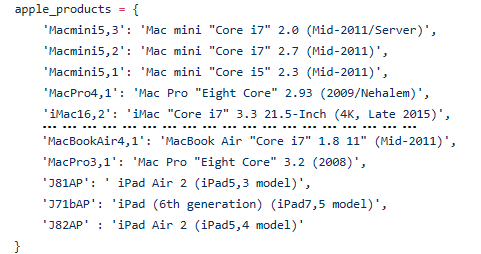
\includegraphics[width=12cm]{015_apple_prod}
	\caption{Dizionario dei modelli di dispositivi Apple\label{fig:apple_prod}}
\end{figure}

Le ultime strutture sono adibite all'analisi e alla scomposizione di \textit{hostname.local} annunciati dai dispositivi nei record di risposta mDNS di tipo A o di tipo AAAA.\\
La prima � un'insieme di \textit{dizionari}, sempre indicizzati dalle Categorie di dispositivi precedentemente descritte, chiamato \textbf{\textit{keyword\_on\_alias}}, all'interno del quale, per ogni categoria, � presente un ulteriore dizionario che contiene le coppie \textit{<chiave, valore>}, dove \textit{chiave} rappresenta appunto la keyword che solitamente � presente negli hostname di quel tipo, e \textit{valore} � una stringa che descrive brevemente quale � il dispositivo che riporta quella keyword nel proprio nome.\\
Le ultime 2, \textbf{\textit{common\_string}} e \textbf{\textit{common\_string\_s}} sono liste ordinate di \qts{stringhe comuni} che solitamente compongono l'hostname.local, e sono utilizzate per \qts{ripulire} la stringa ed ottenere un \textit{nominativo} al quale attribuire il ruolo di \qts{possessore del dispositivo}. Questo processo � stato una conseguenza dello studio dei vari hostnames annunciati nelle reti utilizzate per la cattura di traffico dati in fase di sviluppo, test, e validazione, raccogliendo quindi i pattern di stringhe pi� comuni ed ottenendo dei risultati tutto sommato accettabili in fase di validazione, e identificando nella maggior parte dei casi il nome corretto del possessore del dispositivo.\\

\subsection{run\_test.py}

Modulo utilizzato principalmente in fase di \textit{test} e di \textit{debug}, ma che tutto sommato ne � un \qts{\textit{template}} dal quale se ne pu� ricavare un tutorial di utilizzo dello strumento sviluppato per questo lavoro di tesi.\\

Non � altro che una sequenza di istruzioni, le quali creano un'istanza della classe principale \textit{NetworkLAN}, aprono una serie di file di cattura tramite la funzione offerta da Pyshark \textit{pyshark.FileCapture()} nei 2 rispettivi modi\footnote{[!]Come accennato in precedenza, l'utilizzo di ognuna delle 2 opzioni implica la possibilit� di recuperare facilmente le informazioni di un tipo(mDNS/Dropbox), impossibilitando il recupero delle informazioni dell'altro. Per ulteriori dettagli, riferirsi alla documentazione\cite{web:pyshark} di PyShark reperibile in rete} con cui codifica i pacchetti restituiti: \textit{use\_json=False} per recuperare le informazioni mDNS, e \textit{use\_json=True} per ottenere i dati nei campi dei pacchetti Dropbox db-lsp-disc.

\section{Validazione}

Il processo di validazione approntato per questo Lavoro di Tesi � partito da un'analisi sulla completezza riguardo il materiale reperibile a proposito dei protocolli presi in esame, quali mDNS e DB-LSP-DISC, e rispetto ai risultati ottenuti nei test.\\

Per quanto riguarda lo studio del protocollo \textit{mDNS}, il punto di partenza � stato l'analizzare numerosi \textit{RFC} a riguardo, a partire dalla definizione dello \textit{standard} del protocollo, reperibile in RFC6762\cite{mDNS}, nel quale viene appunto fornita una traccia dello Standard mDNS. In questo documento ne vengono descritti i comportamenti, come i meccanismi di \textit{query-response}, le modalit� con cui i dispositivi che utilizzano il protocollo si annunciano in rete, si scambiano dati. Inoltre viene riportato il dettaglio delle informazioni che se ne possano ricavare, il formato con cui vengono diffuse, e i campi del pacchetto nei quali reperirle.\\
Altri RFC analizzati riguardo mDNS sono stati \textit{RFC-6973}\cite{rfc6973} e \textit{RFC-8386}\cite{rfc8386}, nei quali sono state fatte numerose considerazioni riguardo la \textit{Privacy} dei protocolli Broadcast e Multicast, e pi� in generale del traffico Internet. Questi documenti si possono considerare come lo spunto principale dal quale ne � scaturito questo lavoro di Tesi, in quanto ne � effettivamente una constatazione di quali informazioni si riescono ad acquisire dai protocolli Broadcast/Multicast.\\

Per quanto riguarda i tipi di servizi annunciati tramite i record \textit{DNS-SD}, nel corso dello studio preliminare e raccolta di informazioni, � stato analizzato l'elenco dei \qts{\textit{servizi dichiarati}} dall'organizzazione \textit{Internet Assigned Numbers Authority}, conosciuto come IANA\cite{IANA}. Per ovvie ragioni tempo, non sono stati visionati ed utilizzati tutti i servizi dichiarati in questa raccolta, anche dato che la probabilit� di imbattersi in molti di loro � molto bassa, e per quasi la totalit� sono servizi s� \textit{dichiarati} in questo elenco, ma sono servizi proprietari, e i loro comportamenti e interazioni fra chi li annuncia e chi ne usufruisce molto spesso non sono documentati. Per questi motivi, ci si � affidati ad alcune \qts{liste pi� ristrette} di servizi, le quali riportavano quelli \qts{pi� comunemente utilizzati}. 
Per ampliare queste liste e rendere questo studio \textit{completo}, per lo meno per quanto riguarda gli ambienti sui quali � stata testata la funzionalit� del tool sviluppato per questo studio, � stata raccolta documentazione anche riguardo tutti quei servizi riscontrati nelle catture del traffico di rete, utilizzate in fase di sviluppo.\\
Questo approccio, per quanto di primo impatto possa considerarsi impreciso e incompleto, ha prodotto degli ottimi risultati in fase di test e validazione, riuscendo a catalogare \textit{correttamente} la totalit� dei dispositivi rilevati in questa fase, provando la bont� dell'elaborato.\\
In sintesi, l'iter che ha portato al \qts{popolamento} degli insiemi di servizi annunciati tramite mDNS-DS � stato: partire da un elenco di servizi comunemente usati, e in fase di sviluppo e di test, aggiunti man di mano tutti quelli nuovi incontrati e che non ne facevano parte inizialmente, utilizzandoli nella categorizzazione dei dispositivi dopo uno studio a riguardo sul singolo servizio da aggiungere.\\

La raccolta di materiale inerenti ai pacchetti di Dropbox \textit{Discovery} � partita dall'analisi del documento/guida \qts{\textit{Namespace Guide}}\cite{web:dropboxNS}, reperibile online sul sito della compagnia Dropbox nella sezioni sviluppatori. Tale documento riporta la natura e l'implementazione dei \qts{Namespaces}, fornendo dettagli su come sfruttate tali informazioni ai nostri scopi: scoprire le relazioni fra i dispositivi presenti nella rete locale.\\
La guida copre argomenti avanzati relativi a cartelle e file condivisi di varia natura, dalle \textit{Shared Folders}, \textit{Team Folders} e \textit{Team Spaces \& Member Folders} per i Business Accounts. Lo scopo del documento � quello di fornire una guida all'utilizzo dell'API di Dropbox, quindi non esattamente inerente al nostro lavoro, ma fornisce comunque un'ottima spiegazione riguardo al \qts{cosa sono i namespaces}, da cosa vengono ricavati, cosa rappresentano, e soprattutto quali informazioni si possono dedurre da essi.\\

Riguardo la completezza delle informazioni sulle quali si basa l'analisi del tool, si pu� concludere che i dati raccolti rappresentano sicuramente la totalit� delle informazioni ricavabili dal traffico di una rete locale. Questo � mutuato dal fatto che se, come nelle reti di calcolatori spesso accade, viene perso un pacchetto, o magari non viene rilevato dallo strumento di cattura, il pacchetto viene comunque ritrasmesso ogni 30 secondi circa, come prevedono i protocolli presi in esame(mDNS e DB-LSP-DISC). Quindi effettuando una cattura di pochi minuti si ha la certezza di aver raccolto tutte le informazioni che possono circolare in quel dato momento all'interno di una rete locale.\\
Anche per quanto riguarda il recupero e la codifica degli stessi dati non � stato un problema, in quanto tutte le informazioni dei protocolli analizzati vengono trasmesse in chiaro e a tutti i dispositivi connessi, ed � proprio uno dei punti di partenza di questo studio. Come gi� accennato in precedenza, il punto di forza di questa analisi � proprio la \qts{discrezione} e la facilit� con la quale si ottengono informazioni private dai dispositivi.\\

Analizzando il modo con cui vengono classificati i dispositivi, si evince anche l'affidabilit� della classificazione, giustificata da varie considerazioni e derivata da pi� elaborazioni sequenziali dei dati di natura differente, portando quindi a convergere verso una corretta deduzione sul tipo di dispositivo.\\
Uno dei punti di forza della corretta classificazione � appunto il grado \qts{affidabilit�} associato ad ogni informazione in base al quale il tool assegna una \textit{classe} rispetto che un'altra ad un dispositivo. Ad esempio, se un nodo riporta nel suo hostname una keyword evocativa, che potrebbe indurre ad una classificazione corretta come errata, non gli viene associato direttamente quella classificazione, ma si va a verificare tale informazione analizzando i servizi che esso annuncia, e quindi solo allora viene etichettato il dispositivo con la corretta classe. Anche l'informazione riguardante \textit{modello} e \textit{versione OS} viene comunque verificata analizzando gli altri servizi offerti.\\
Anche la scelta delle keyword non � casuale, ma bens� � frutto di numerose catture e verifiche in fase di sviluppo, riportando solo le parole chiave che effettivamente potessero essere usate come discriminanti per i vari dispositivi, e solo dopo un'attenta verifica che quella determinata keyword appartenga effettivamente a quella particolare categoria o a quel particolare dispositivo nello specifico.\\

Per validare tutte queste considerazioni, oltre che ad eseguire il tool in ambienti eterogenei e che presentassero un p� la totalit� delle situazioni che si possano riscontrare nella realt�, sono stati sia raccolti dati in ambienti controllati e \qts{conosciuti}, quindi avendo ben presente le tipologie di dispositivi che facessero parte della rete locale. La validazione quindi � avvenuta sia verificando di persona, direttamente sul dispositivo identificato, che l'analisi effettuata su di esso fosse corretta categorizzandolo nel giusto modo, sia constatando, dove fosse stato possibile dedurre correttamente nome e cognome del proprietario che in quel momento lo utilizzava, l'effettiva presenza di quella persona.

\subsection{Analisi dei Risultati}

Di seguito vengono riportati alcuni risultati, omettendo opportunamente alcune informazioni ai fini di tutelare la sicurezza e la privacy di persone e reti nella quale � stata effettuata la cattura.\\
\begin{figure}[h]
	\centering
	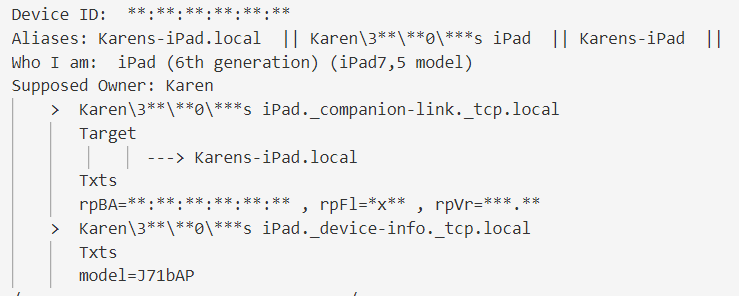
\includegraphics[width=\linewidth]{001_ipad}
	\caption{Esempio di analisi di un dispositivo\label{fig:ipad}}
\end{figure}

In questo esempio si nota come sia il nome, sia la diffusione del record \qts{\_device-info} vengono utilizzati per dedurre Tipo del dispositivo e \qts{ipotetico possessore}.\\

Un'altro esempio che vale la pena osservare � il seguente, nel quale viene rilevato un dispositivo mobile, dando addirittura un \textit{Cognome} al possessore(non riportato interamente per motivi di privacy).
\begin{figure}[htbp]
	\centering
	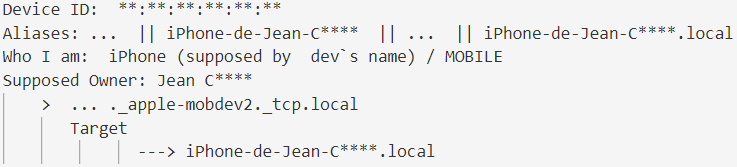
\includegraphics[width=\linewidth]{002_iphone}
	\caption{Dispositivo mobile\label{fig:iphone}}
\end{figure}
\\
Interessante notare il fatto che non � solo l'\textit{hostname} che attribuisce la categoria al dispositivo, ma tale supposizione viene comunque confermata dal servizio \textit{\_apple-mobdev2}, che rientra nella categoria di tutti quei servizi che vengono diffusi dai dispositivi mobili Apple.\\

Di completamente differente categoria � la rilevazione di una stampante, la quale oltre che al modello e produttore, diffonde numerose informazioni \qts{private}, che magari un eventuale intruso nella rete potrebbe sfruttare.
\begin{figure}[htbp]
	\centering
	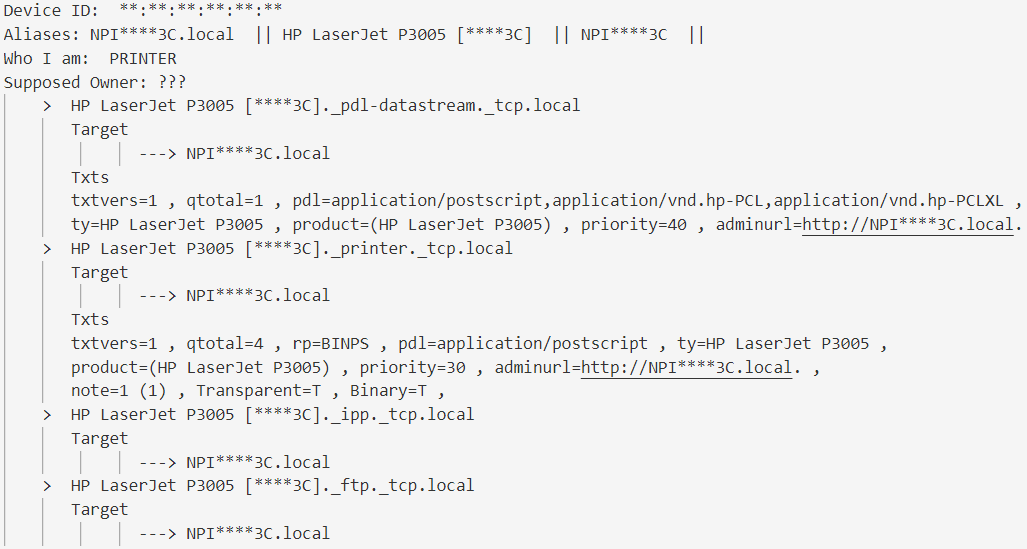
\includegraphics[width=\linewidth]{004_printer}
	\caption{Stampante collegata in rete\label{fig:printer_info}}
\end{figure}\\

Il prossimo esempio dimostra la validit� con cui sono state suddivise le categorie di servizi che ogni tipologia di dispositivo annuncia, che anche senza l'ausilio del rilevare la keyword \qts{\textit{NAS}} all'interno dell'hostname, ha correttamente identificato il nodo della rete come NAS analizzando solo i servizi dichiarati dalla macchina.
\begin{figure}[htbp]
	\centering
	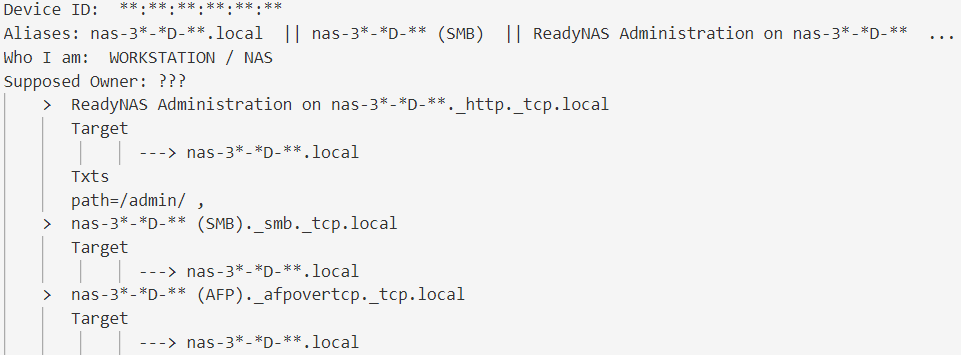
\includegraphics[width=\linewidth]{006_nas}
	\caption{Dispositivo adibito a Network Attached Storage\label{fig:nas}}
\end{figure}

Nel complesso, in tutti i file di cattura utilizzati per testare il tool sviluppato per questo lavoro, sono stati rilevati un totale di 160 dispositivi classificandoli correttamente 156, e restando nell'incertezza, a causa di informazioni non sufficientemente caratterizzanti, con solo 4 dispositivi. Sono state quindi rilevati: 99 Workstation, di cui 16 Personal computer Apple, e ben 88 dei quali aventi Dropbox in esecuzione in quel momento; 15 NAS, di cui 7 Time Capsule; 17 dispositivi Mobili, suddivisi in 5 iPhone, 7 iPad e 7 Android; 29 Stampanti, rilevando 2 dispositivi che ne condividevano almeno una.\\

Passando invece ad analizzare i risultati ottenuti riguardo l'elaborazione delle informazioni recuperate dai pacchetti Dropbox, ci troviamo di fronte un'ampia rete di collegamenti fra i dispositivi(e in un certo senso anche fra gli utenti che abitualmente utilizzano quella rete locale). I dati riportati in figura sono stati opportunamente censurati per motivi di privacy, quindi riportano soltanto le ultime 3 cifre che compongono il MAC-Address del dispositivo.
\begin{figure}[htbp]
	\centering
	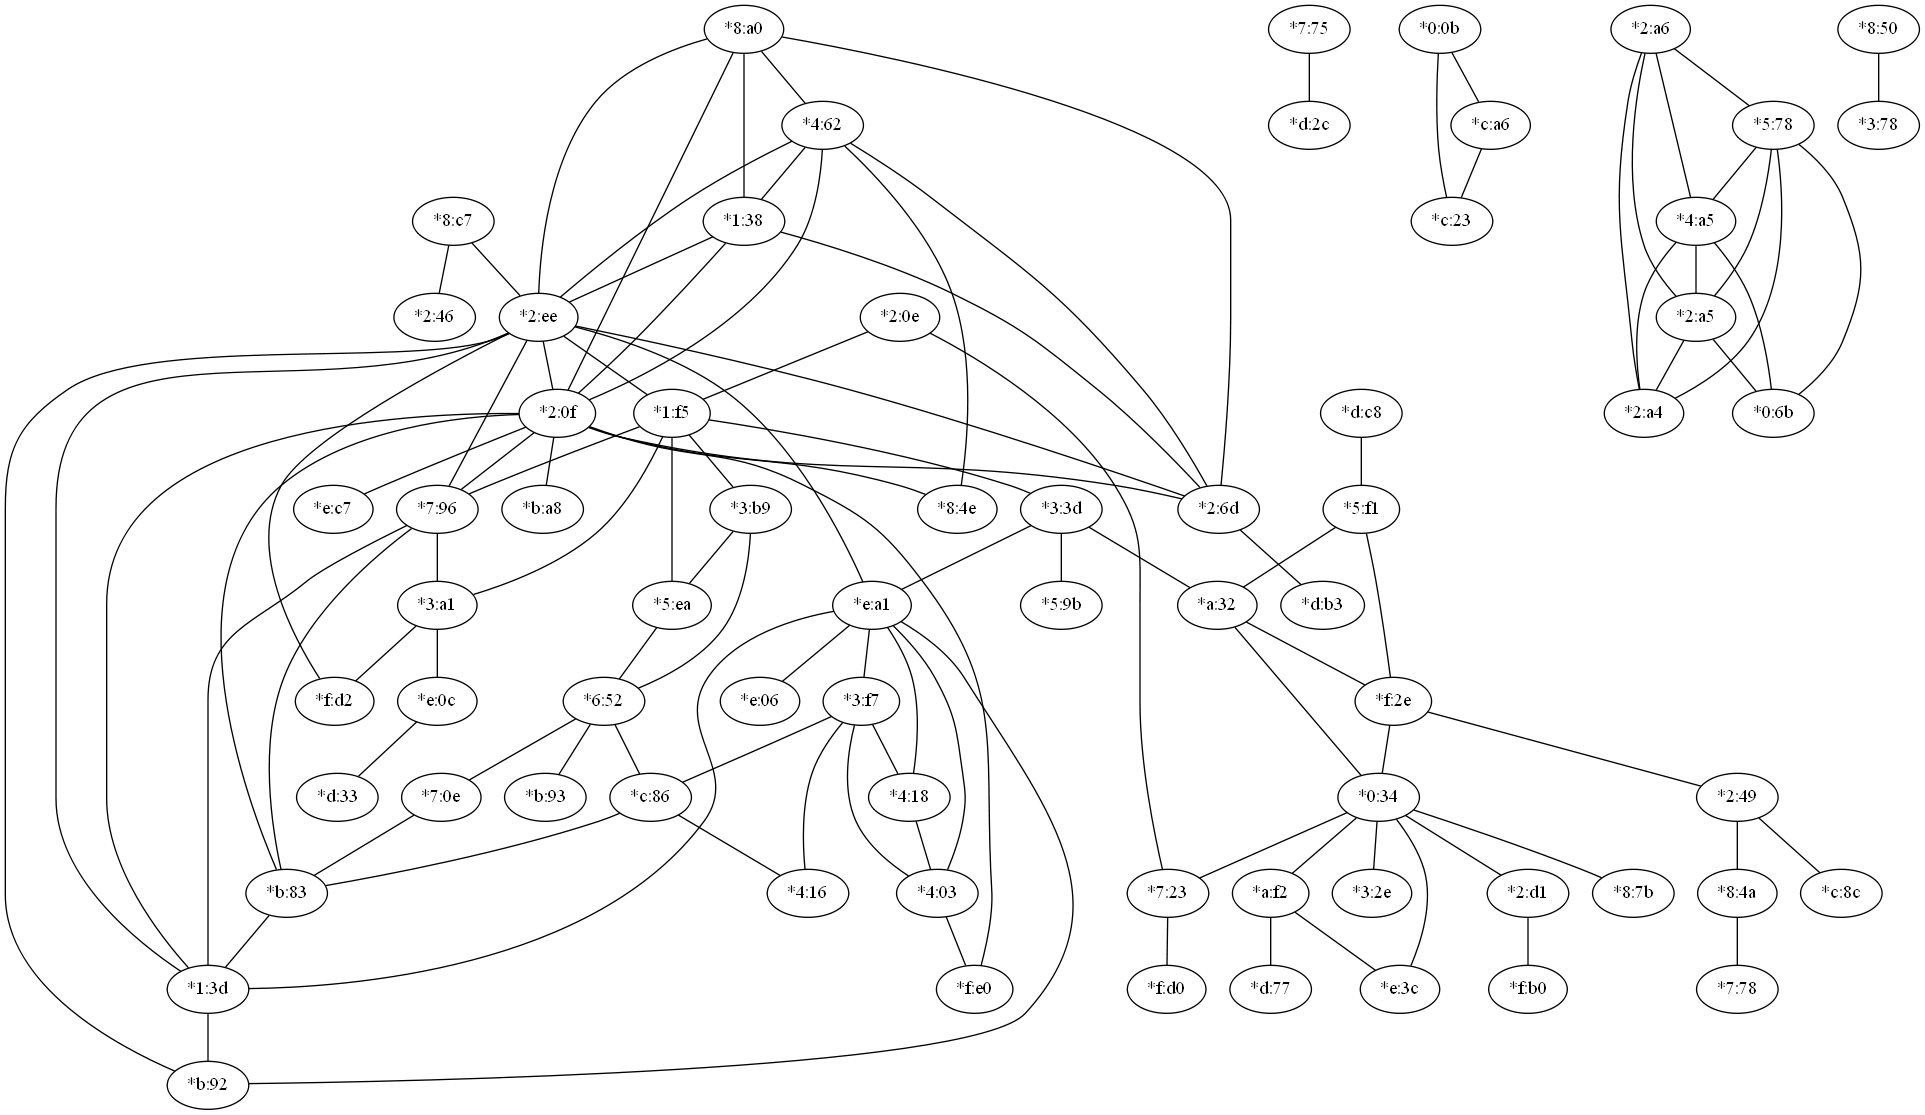
\includegraphics[width=\linewidth]{007_graficoDB}
	\caption{Relazione fra i dispositivi che utilizzano Dropbox\label{fig:grafDB}}
\end{figure}

Per validare la correttezza del risultato ottenuto, sono state condotte delle verifiche di persona direttamente sui dispositivi aventi quel determinato MAC-Address, constatando che effettivamente in quel momento ci fossero delle cartelle condivise tramite Dropbox, e che il collegamento fra le macchine fosse legittimo, e quindi rappresentasse effettivamente \qts{la cartella condivisa tra i 2 host}.\\

Analizzando il grafo, si possono fare numerosissime supposizioni sulla topologia della rete, in particolare sui punti di snodo con il maggior numero di collegamenti: quei nodi potrebbero benissimo rappresentare un server sul quale risiedono dei dati condivisi da un gruppo di lavoro, o ancora quei dispositivi potrebbero essere dei PC che magari appartengono ad un capogruppo, il quale per avere una panoramica dell'intero lavoro, fa condividere ai singoli partecipanti la loro cartella dove viene raccolto il materiale sul quale stanno lavorando.\\

Quest'ultima osservazione potrebbe dar vita ad altre supposizioni, come per esempio raggruppare aree di nodi per tentare di identificare i gruppi di lavoro ed ottenere magari informazioni aggiuntive o del tutto mancanti riguardo alle macchine rilevate dal nostro tool.\\
Altre informazioni che si possono ricavare sono le relazioni \textit{personali} fra gli utenti proprietari dei dispositivi. Se per esempio grazie all'analisi mDNS, sempre effettuata dallo strumento sviluppato per questo lavoro di Tesi, � stato possibile ricavare un nome per il possessore del dispositivo, si possono rivelare le interazioni che quell'utente ha con altre persone o dispositivi all'interno della rete locale.\\

Per concludere, sicuramente si possono accrescere il numero di informazioni ottenute dalle comunicazioni Broadcast e Multicast, incrementando il numero di protocolli analizzabili che trasmettono, per mezzo di questi canali, informazioni in \qts{chiaro} e personali, relative ai dispositivi e ai loro utilizzatori, ma per questo lavoro di tesi � stato deciso di utilizzare solo i dati raccolti da mDNS e dai pacchetti DB-LSP-DISC. Per quanto riguarda tutti gli altri, possono essere un'ottimo spunto per estendere il tool di analisi, e quindi rimandati per lavori futuri.
	%%%%%%%%%%%%%%%%%%%%%%%%%%%%%%%%%%%%%%%%%%%%%%%%%%%%%%%%%%%
% Capitolo 5

\chapter{Conclusioni e Lavori Futuri}
\label{ref:Conclusioni}

\section{Lavori futuri}
Come accennato in precedenza, la scelta stessa del linguaggio di programmazione(Python), per sviluppare il tool per l'analisi della rete locale, � stata fatta per rendere questo lavoro di Tesi come un punto di partenza, da estendere e migliorarne le capacit� di deduzione riguardo le reti di calcolatori e i dispositivi connessi ad esse.\\
Anche la considerevole quantit� di protocolli ed applicativi che fanno uso dei canali di Broadcast e Multicast � un'ottimo spunto dal quale potrebbe scaturire il proseguimento nello sviluppo di questo Elaborato.\\

Un esempio potrebbe essere quello di estendere il tool aggiungendo la capacit� di analizzare dati provenienti da protocolli come NetBIOS o \textit{Microsoft Windows Browser Protocol}, incrementando le informazioni acquisite, e quindi andare ad identificare tutti quei dispositivi che non usufruiscono dei protocolli gi� inclusi nello strumento di analisi, e che quindi non vengono \qts{rilevati} da quest'ultimo.\\

Un'altra idea per estendere questo lavoro � incrementare la capacit� di analisi del tool aggiungendo la possibilit� di riconoscere \textit{nomi} di persone, dispositivi, e quant'altro possa rivelare ulteriori informazioni a partire dalle stringhe reperite dagli hostnames dei nodi della rete. Un punto di partenza sarebbe aggiungere ulteriori dizionari di keyword da utilizzare per identificare la tipologia di dispositivo che le integra nel proprio hostname. O ancora, aggiungere la capacit� di reperire in rete, tramite appositi servizi o API, elenchi aggiornati con i nomi, cognomi e diminutivi di persone comunemente usati, e quindi riuscendo con maggiore facilit� e precisione ad attribuire un proprietario ad un dato dispositivo.\\

Una capacit� che per motivi di tempo non � stata sviluppata, � quella di dettagliare ulteriormente la caratterizzazione dei dispositivi andando ad analizzare i campi \textit{TXT} di tutti quei servizi che includono informazioni riguardo le caratteristiche Hardware e Software del dispositivo, non limitandosi a quelle dei record \textit{ \_device-info } annunciati solo dai dispositivi Apple.\\
I servizi che li diffondono sono numerosi, a partire dai protocolli di stampa, come \textit{\_ipp} che forniscono moltissimi dettagli sulla stampate di rete, fino ad arrivare a servizi che fungono da \textit{appoggio} a protocolli e applicativi proprietari, come ad esempio \textit{\_nomachine} che diffonde informazioni riguardo la macchina che si rende disponibile al controllo di desktop remoto, fornendo informazioni come: \textit{OS=Ubuntu 18.04.1 LTS} e \textit{uuid=\dots} .\\

Un'altra funzionalit� che potrebbe incrementare il numero di informazioni estratte dai campi mDNS � quella di effettuare delle \qts{query attive} per il discovery di tutti quei dispositivi che, s� offrono servizi, ma che magari a causa di comportamenti pi� conservativi non divulgano informazioni a riguardo se non direttamente interpellati. 
Con questa utilit� quindi si va a stimolare in maniera diretta il nodo in questione, incrementando quindi le informazioni riguardo i servizi offerti.\\

\section{Conclusioni}

Questo studio riguardo la raccolta di informazioni su reti locali e dispositivi ad esse connessi si � rivelato pi� soddisfacente, considerata la quantit� di informazioni a cui si � avuto accesso.\\

L'obiettivo di \qts{anonimato} e discrezione per quanto la raccolta dati, e lo strumento utilizzato a tale scopo, � stato pienamente raggiunto, in quanto non � possibile in alcun modo identificare il tool che in quel momento sta catturando ed analizzando i pacchetti che circolano nella rete.
Infatti, lo strumento si limita ad analizzare i pacchetti, e quindi le informazioni in essi contenuti, che vengono recapitati \textit{direttamente} alla macchina sulla quale � in esecuzione, non compiendo alcuna azione che potrebbe rendere visibile l'\textit{attivit� di analisi} della rete.\\

Per quanto riguarda il tipo di informazioni che � stato possibile ricavare dai dati reperiti dalle comunicazioni Broadcast e Multicast, si sono rivelati sorprendenti, svelando dettagli, specialmente per quanto riguarda i dispositivi, decisamente \qts{personali}, e che potrebbero essere sfruttati come punti di debolezza per eventuali attacchi da parte di intrusi nella rete, o utenti \qts{malintenzionati}.\\
Riguardo ai dispositivi, � stato possibile identificare, nei casi pi� fortuiti: modello del dispositivo, e quindi tutte le caratteristiche Hardware di cui dispone, e Sistema Operativo, nonch� versione installata in quel momento, fornendo dettagli del Software che vi � in esecuzione.
Inoltre, sempre riguardo i dispositivi, vengono fornite informazioni sulle periferiche che in quel momento sono a loro connesse, come ad esempio stampanti, scanner, ed altro materiale \qts{da ufficio}.
In casi pi� generici invece, vene comunque identificata correttamente la \textit{Classe} a cui il dispositivo appartiene, grazie ai servizi applicativi che esso offre, fornendo un'idea generica di come vengano sfruttate le reti locali analizzate: per utilizzo \qts{d'ufficio} se vengono rilevate principalmente stampanti, fax e scanner, o magari per il solo accesso alla rete Internet globale, se rilevati principalmente dispositivi mobili, o ancora per un utilizzo \qts{privato} e condivisione di \textit{Media}, se vengono rilevati numerosi dispositivi atti a condividere file, musica, streaming video e audio, e quant'altro di simile.\\
Tutte queste informazioni riguardo i dettagli dei dispositivi, potrebbero essere sfruttate per \textit{indagini di mercato} da tutte quelle aziende che lavorano nel settore, e quindi sfruttando le \qts{abitudini} degli utenti di una determinata rete locale, potrebbero ricavare informazioni utili ai loro scopi, come intraprendere o meno determinate scelte riguardo la vendita e promozione dei propri prodotti.\\

Per quanto riguarda gli utenti, le persone fisiche che quindi in alcuni casi possiedono il dispositivo, l'informazione pi� personale che si riesce a ricavare da questo studio sono il \textit{nome} e \textit{cognome}.
Per quanto possa a prima vista non sembrare particolarmente rilevante, sono comunque informazioni che appartengono alla sfera privata degli utenti, e quindi visto il modo con cui vengono diffuse.
Questo offre un ottimo spunto di riflessione su come i nostri dati personali vengono utilizzati, e magari dare maggiore consapevolezza dei rischi che si corre utilizzando determinati dispositivi, servizi o tecnologie che a prima vista risultano estremamente comode, ma che tutto sommato comportano degli svantaggi e un prezzo da pagare per quella comodit�: le proprie informazioni.\\

Sempre restando nella \textit{sfera privata} degli utenti, le informazioni ricavate dai pacchetti Dropbox sono ancor pi� rilevanti.
Di fatto, non solo svelano dettagli delicati riguardo la topologia della rete, ma bens� rivelano anche informazioni inerenti alle interazioni sociali che si hanno fra gli utilizzatori di tali reti locali.\\
Queste informazioni possono dare inizio a numerosissime supposizioni a riguardo: a partire dal dedurre quali sono i gruppi di lavoro con i quali vengono organizzate le attivit� di un'azienda, o ancora i ruoli che ricoprono gli utenti che fanno parte di una determinata organizzazione; pi� semplicemente, possono rivelare le relazioni private che incorrono fra i possessori dei dispositivi, ad esempio: se 2 utenti di 2 dispositivi condividono una cartella o dei file, molto probabilmente hanno una qualche sorta di interazione, o per lo meno si conoscono.\\

Ma tutte le informazioni scaturite da questo studio, come possono essere utilizzate? chi potrebbe essere interessato a sfruttarle?\\
Oltre che ad utilizzi dannosi o con il fine di \qts{invadere} la sfera privata degli utenti per scopi di Marketing, questo � un prezioso strumento per conoscere la propria rete locale, e quindi attuare azioni atte a contrastare queste intrusioni.
In primo luogo potrebbero essere usate per incrementare il livello di sicurezza, magari impedendo completamente la circolazione di tali informazioni, o quanto meno restringerle a determinati nodi, suddividendo la rete locale in sotto-reti autonome, e quindi relegandone il traffico all'interno, dato che le comunicazioni Broadcast e Multicast sono limitate alla rete locale di cui fanno parte.\\
Un'altro utilizzo sarebbe quello di monitoraggio di una rete locale, tenendo traccia di quali dispositivi vengono connessi, quali utenti ne fanno parte, e magari rilevando accessi indesiderati da parte di utenti non autorizzati.\\
In fine, pi� semplicemente, queste informazioni potrebbero rendere consapevoli gli utenti di quali dati rendono disponibili, e quindi dare la possibilit� di scegliere le azioni da compiere a riguardo, da un semplice cambio di \textit{hostname}, a magari interrompere l'utilizzo di determinati servizi o tecnologie in favore di altre che offrono gli stessi vantaggi con una maggiore attenzione riguardo i dati diffusi in rete.

	% === Bibliografia =======================================
  \newpage
  \bibliographystyle{plain}
  \bibliography{bibliografia}
  
	% === Appendici ==========================================
	\appendix
	%%%%%%%%%%%%%%%%%%%%%%%%%%%%%%%%%%%%%%%%%%%%%%%%%%%%%%%%%%%
% Appendice A

\chapter{Titolo dell'appendice}
\label{ref:appA}

Se lo si ritiene necessario, scrivere una o pi� appendici.
	%%%%%%%%%%%%%%%%%%%%%%%%%%%%%%%%%%%%%%%%%%%%%%%%%%%%%%%%%%%
% Appendice B

\chapter{Titolo dell'appendice}
\label{ref:appB}

Se lo si ritiene necessario, scrivere una o pi� appendici.

\end{document}
